\documentclass[review,1p]{elsarticle}

% ---------- Journal target ----------
\journal{Information Sciences}

% ---------- 通用包 (elsarticle 不自带, 全部显式 import) ----------
\usepackage{amsmath}
\usepackage{amssymb}
\usepackage{amsthm}
\usepackage{graphicx}
\usepackage{booktabs}
\usepackage{xcolor}
\usepackage[hyphens]{url}
\usepackage[hidelinks]{hyperref}
\usepackage{multirow}
\usepackage{enumitem}
\usepackage{natbib}
\graphicspath{{figures/}}

% ---------- citation style: author-year (compatible with existing \citep / \citet) ----------
\bibliographystyle{elsarticle-harv}

% ---------- theorem environments ----------
\newtheorem{lemma}{Lemma}
\newtheorem{theorem}{Theorem}
\newtheorem{proposition}{Proposition}
\newtheorem{definition}{Definition}

% ---------- 自定义命令 ----------
\newcommand{\R}{\mathbb{R}}
\newcommand{\bv}{\bar{v}}

\begin{document}

% Looser linebreaking for long 	exttt{...} paths and inline math
\sloppy
\emergencystretch=3em
\tolerance=9999
\hyphenpenalty=50
\hbadness=10000


\begin{frontmatter}

% ---------- Title ----------
\title{Geometric Post-Processing for Weak-Baseline LLM Embeddings: PQ-Chamfer Distance, Graph Regularization, and a Supervised Per-Query Fusion Predictor}

% ---------- Author (anonymized for double-blind review) ----------
\author{Anonymous}
\address{Anonymous Institution}
\ead{anonymous@example.com}

% ---------- Abstract ----------
\begin{abstract}
General-purpose large language model (LLM) hidden states, when used directly for retrieval via mean-pooled centroid cosine, give baselines weaker than retrieval-trained dense encoders. We ask whether \emph{geometric post-processing}---a hybrid pipeline composing parameter-free distance and smoothing operators with a supervised per-query fusion-weight predictor---can close part of this gap on weak-baseline LLM embeddings. The geometric operators (PQ-Chamfer distance and graph Laplacian smoothing) are parameter-free at inference; the per-query fusion weight $\lambda$ is learned by a gradient-boosted regressor under a 50/50 train/test split, with cross-corpus leave-one-out audit confirming transferable rather than per-corpus-overfit signal.

We introduce a two-stage geometric reranking pipeline on token-level point clouds extracted from a frozen Qwen3-8B-Q4. Stage~1, \textbf{PQ-Chamfer distance}, exploits the product-quantization decomposition $\mathbb{R}^{4096} = \bigoplus_{s=1}^{64} \mathbb{R}^{64}$, computes exact per-subspace cosine distances, and averages them, breaking concentration of measure without quantization error. Stage~2, \textbf{graph Laplacian smoothing} on a $k$-NN document graph built from PQ-Chamfer distances, propagates relevance across inter-document structure. The per-query fusion weight is learned by a supervised gradient-boosted regressor (GBM-11) under a 50/50 train/test split.

On five non-Quora BEIR corpora, the pipeline lifts the Qwen3-8B token-centroid cosine baseline by $+20.9\%$ (SciFact) to $+157.4\%$ (FiQA) NDCG@10. Paired bootstrap against per-corpus oracle gives $p<0.001$ on four corpora and $p<0.005$ on SciFact (Cohen's $d$ 0.20--0.72). Against six audited baselines on identical splits (Ours \textbf{first} on SCIDOCS, \textbf{second} on ArguAna, \textbf{fourth} on NFCorpus and FiQA, \textbf{last} on SciFact); the pipeline does not dominate the baseline grid as a whole but does outperform PLAID (state-of-the-art late-interaction) on ArguAna ($+36.0\%$), SCIDOCS ($+37.7\%$), and FiQA ($+11.7\%$). Theorem-grounded analysis (PQ subspace discrimination bound + curse-of-orthogonality + Laplacian convergence; \S\ref{subsec:theory}) explains the niche pattern: the pipeline excels on weak-cosine corpora and trails when same-encoder cosine $\gtrsim 0.45$. This positions the contribution as \emph{theory-grounded geometric post-processing on weak-baseline LLM embeddings}. A vector-provenance audit during revision flipped a key cross-model finding: under per-(model,corpus) tuning, smoothing on BGE-M3 changed from $+6.2\%$ NFCorpus gain (pre-audit) to $-1.50\%$ (audited rebuild after fixing $19.93\%$/$18.62\%$ silently-zero-encoded NFCorpus/SciFact documents); we accordingly re-position the smoother to a weak-baseline LLM-embedding niche (cross-model unified default helps $2/10$ corpus-model cells in our $5\times2$ grid). This work additionally documents 21 falsified approaches under uniform provenance disclosure (11 complete raw logs; 7 retrospectively reconstructed; 3 a priori category errors as design-space exclusions; per-entry flags in Supplementary~A.3) organised into a three-class failure-mechanism taxonomy. The full pipeline cost \$47 on a single consumer GPU.
\end{abstract}

% ---------- Keywords ----------
\begin{keyword}
dense retrieval \sep LLM embeddings \sep product quantization \sep graph Laplacian smoothing \sep BEIR benchmark
\end{keyword}

\end{frontmatter}

% ============================================================
\section{Introduction}
\label{sec:introduction}
% ============================================================

Retrieval-Augmented Generation (RAG) has become the dominant paradigm for grounding large language models in external knowledge \citep{lewis2020rag,guu2020realm}. The standard RAG pipeline employs a bi-encoder to map queries and documents into a shared embedding space, then ranks candidates by cosine similarity. Let $\mathbf{v}_q \in \R^d$ and $\mathbf{v}_i \in \R^d$ denote the query and document embeddings, respectively:
\begin{equation}
\label{eq:cosine}
\text{score}(d_i) = \frac{\mathbf{v}_q \cdot \mathbf{v}_i}{\|\mathbf{v}_q\| \, \|\mathbf{v}_i\|}
\end{equation}

This formulation has two fundamental limitations. First, it represents each document as a \textit{single point} in $\R^d$, conflating diverse semantic facets into one centroid. Second, it scores each document independently, ignoring inter-document structure---topic clusters, semantic neighborhoods, and distributional patterns---that the retrieved set collectively encodes.

Existing parameter-free remedies do not address these two limitations directly. Query-rewriting methods such as HyDE~\citep{gao2023hyde} and Query2Doc~\citep{wang2023query2doc} alter the query but leave the document representation intact, so cosine concentration in $\R^d$ persists at scoring time. Sparse--dense fusion with BM25~\citep{robertson2009bm25} adds lexical signal but does not recover sub-document structure, and shares cosine's pointwise scoring assumption on the dense side. Pseudo-relevance feedback (PRF) over dense embeddings~\citep{li2023ance-prf} expands the query in embedding space, again inheriting concentration of measure. Late-interaction architectures such as ColBERT and ColBERTv2~\citep{khattab2020colbert,santhanam2022colbertv2} explicitly preserve token-level structure but require dedicated training of a token-aware encoder, contradicting the operator-level parameter-free regime we target. The gap we identify, therefore, is the absence of a method that (a)~exploits the token-level geometry of frozen general-purpose embeddings and (b)~scores documents jointly through inter-document structure without retrieval-specific encoder training (the supervised fusion-weight predictor in our pipeline trains only an 11-dimensional regressor, not the encoder).

This gap is addressed by treating documents as point clouds rather than points \citep{anonprior2026a}. The per-token hidden states of a language model form a cloud in embedding space whose spread, density variation, and subspace projections carry semantic information that a single centroid discards. Two design questions follow: what distance metric is appropriate between document point clouds, and how can inter-document structure be incorporated without the cost of cross-encoder inference? Both are answered with parameter-free geometric operations: PQ-Chamfer distance for the first, graph Laplacian smoothing for the second.

\textbf{Relation to prior versions.} This paper extends a prior anonymised research program \citep{anonprior2026a,anonprior2026b}. Earlier iterations explored convection-diffusion equations and sentence-level point clouds. The present work abandons the convection-diffusion narrative---experimentally falsified across five independent validations (Section~\ref{subsec:falsification})---and reorganises the framework around token-level point clouds, PQ-Chamfer distance, and graph Laplacian smoothing.

\subsection{Contributions}
\label{subsec:contributions}

We present three substantive contributions for retrieval over frozen general-purpose LLM token clouds.

\textbf{(N1) PQ-without-quantization as exact subspace-averaged distance.} Product quantization is canonically a compression primitive paired with $K$-means codebooks; we keep the subspace decomposition $\R^{4096} = \bigoplus_{s=1}^{64} \R^{64}$ and \emph{drop} the codebook, computing exact per-subspace cosine distances and averaging. Theorem~\ref{thm:pq-discrim} establishes a closed-form $\sigma_{\rm sub}/\sigma_{\rm full} = \sqrt{M/(1+(M-1)\rho)}$ discrimination ratio on anisotropic embedding spaces, validated empirically on $M \in \{16, 32, 64, 128\}$ (Section~\ref{subsec:concentration-measurement}, $6$--$14\%$ relative error to closed-form prediction across all four $M$ values). The construction inverts ColBERTv2/PLAID's quantize-then-rank trade-off (variance inflation without quantization error).

\textbf{(N2) Graph Laplacian on a point-cloud-distance KNN graph.} Standard graph-rerank methods (G-RAG, GAR) build edges from single-vector centroid similarities; we build edges from PQ-Chamfer between document token clouds. Theorem~\ref{thm:laplacian-cluster} proves convergence of the smoothing iteration to the cluster-hypothesis fixed point at rate $(1-\alpha\lambda_2)^t$, formalising the over-smoothing transition observed empirically at $T \gtrsim 20$.

\textbf{(N3) Curse-of-orthogonality bound and a three-class falsification taxonomy with cross-corpus generalization audit.} Theorem~\ref{thm:curse-orthogonality} formalises an $O(1/\sqrt{d})$ signal-to-noise upper bound for any directional-transport mechanism in $\R^d$; the bound, combined with two further bounds (aggregation pathology, saturation), explains why 21 systematically-falsified approaches fail. We further audit the supervised per-query fusion-weight predictor (GBM-11) for oracle leakage via leave-one-corpus-out (LOCO) transfer (Section~\ref{subsec:adaptive-lambda}): cross-corpus GBM-11 (trained on 4 corpora, tested on the 5th) achieves macro NDCG@10 $0.4091$ vs.\ in-corpus $0.4072$ ($+0.47\%$ macro), demonstrating transferable task-level signal rather than per-corpus overfitting.

The pipeline is positioned along a \textbf{baseline-strength gradient}: weak frozen-LLM cosine baselines (NDCG@10 $\sim 0.17$--$0.45$) yield large geometric gains, while strong retrieval-trained baselines ($\sim 0.31$--$0.64$) yield mixed gains. Code, indices, and the full falsification log are released at an anonymous repository (URL provided to reviewers separately to preserve double-blind review).

\subsection{Research Objectives}
\label{subsec:research-objectives}

This study addresses the following research questions:
\begin{enumerate}
\item \textbf{RQ1:} Can parameter-free geometric operations (PQ-Chamfer distance and graph Laplacian smoothing), composed with a supervised per-query fusion-weight predictor, on general-purpose LLM hidden states improve dense retrieval quality?
\item \textbf{RQ2:} How does the improvement transfer across different frozen embedding architectures (Qwen3-8B-Q4, BGE-M3, BGE-large-en-v1.5), and what are the boundaries of cross-encoder applicability under per-(corpus, model) tuning?
\item \textbf{RQ3:} At what computational cost can these improvements be achieved compared to training specialized retrieval models?
\end{enumerate}

% ============================================================
\section{Literature Review}
\label{sec:related}
% ============================================================

We position our work within five strands of prior research and identify the regime in which our design choices are, to our knowledge, new.

\textbf{Trained multi-vector retrieval.} ColBERT~\citep{khattab2020colbert} introduced late interaction via asymmetric MaxSim on a BERT encoder fine-tuned on MSMARCO; ColBERTv2~\citep{santhanam2022colbertv2} compressed token embeddings via residual quantization with learned codebooks; PLAID~\citep{santhanam2022plaid} accelerated search through centroid pruning. COIL~\citep{gao2021coil}, ME-BERT~\citep{luan2021mebert}, and DESSERT~\citep{engels2024dessert} extend the family. All require (i)~contrastively fine-tuned token-aware encoders and (ii)~asymmetric or dot-product scoring rather than symmetric subspace-averaged cosine.

\textbf{Frozen multi-vector representations.} Sentence-BERT~\citep{reimers2019sbert} pools to a single vector; WMD~\citep{kusner2015wmd} uses EMD on word2vec without graph regularization; BERTScore~\citep{zhang2020bertscore} applies one-directional max-pooling for evaluation. To our knowledge, no prior work computes (a)~symmetric subspace-decomposed Chamfer distance on (b)~frozen general-purpose LLM hidden states for (c)~document retrieval ranking with (d)~an additional inter-document graph regularization step.

\textbf{Recent LLM-based embeddings.} E5-Mistral~\citep{wang2024e5mistral} and GTE~\citep{li2024gte} fine-tune large LLMs on retrieval objectives but collapse per-token clouds via mean pooling. We treat any such encoder as a frozen feature extractor and apply geometric reranking on top; results across Qwen3-8B-Q4, BGE-large-en-v1.5, and BGE-M3 are in Section~\ref{subsec:cross-model}.

\textbf{Late-interaction comparison.} Our pipeline differs from ColBERT family on three axes: (i)~representation source (frozen LLM vs.\ retrieval-trained); (ii)~aggregation symmetry (symmetric subspace-averaged cosine $d_{\mathrm{PQ}} = \tfrac{1}{M}\sum_s \delta_s$ vs.\ asymmetric MaxSim); the subspace average breaks concentration of measure (measured $\sigma_{\rm sub}/\sigma_{\rm full}$ ratio $2.0\times$ on Qwen3-8B); (iii)~inter-document signal via graph Laplacian smoothing on a document KNN graph from PQ-Chamfer distances.

\textbf{Two structural novelties.} \emph{(N1) PQ without quantization, as exact distance.} PQ \citep{jegou2011pq} is canonically a compression primitive paired with per-subspace $K$-means codebooks; we keep the subspace decomposition and drop the codebook, computing exact cosine within each subspace and averaging. ColBERTv2/PLAID inherit the quantize-then-rank trade-off (smaller storage, quantization-error penalty); we invert it (variance inflation without quantization error, full-precision storage). \emph{(N2) Graph Laplacian on a point-cloud-distance KNN graph.} G-RAG~\citep{glass2024grag} and GAR~\citep{macavaney2022gar} build KNN graphs from single-vector similarities; we build it from PQ-Chamfer between document token clouds, giving the smoothing operator a graph topology that respects sub-document structure.

\textbf{LLM-based and graph-based reranking.} RankGPT \citep{sun2024rankgpt}, RankLLM \citep{pradeep2025rankllm}, and AFR-Rank \citep{afrrank2025} achieve strong NDCG@10 but require \$0.01--0.10/query in API costs; \citep{li2025reranking_survey} surveys the evolution. Graph methods span PageRank \citep{page1999pagerank} to diffusion-based RAG \citep{dampanaboina2024diffrag}. PQ systems including FAISS \citep{johnson2021faiss}, ScaNN \citep{guo2020scann}, OPQ \citep{ge2014opq} use subspace decomposition for compression. Chamfer distance \citep{fan2017chamfer} and EMD \citep{rubner2000emd} are dominant 3D point cloud metrics; Chamfer corresponds to unbalanced optimal transport \citep{sejourne2023uot}.

% ============================================================
\section{Methodology}
\label{sec:method}
% ============================================================

\subsection{Document Point Cloud Representation}
\label{subsec:point-cloud}

For a pretrained language model $\mathcal{M}$ (Qwen3-8B, $d = 4096$), document $d_i$'s last hidden states (\texttt{--pooling none}) form the point cloud $\mathcal{P}_i = \{h_{i,1}, \ldots, h_{i,n_i}\} \subset \R^d$; queries form $\mathcal{P}_q$ analogously. NFCorpus average: ${\sim}356$ tokens/doc, ${\sim}6$ tokens/query, 14\,GB SQLite. The centroid $\bv_i = \tfrac{1}{n_i}\sum_j h_{i,j}$ serves as the single-vector representation for initial retrieval and coarse filtering.

\subsection{PQ-Chamfer Distance}
\label{subsec:pq-chamfer}

PQ-Chamfer distance is defined in four stages, presented incrementally below: (i) subspace decomposition of the ambient embedding space; (ii) Chamfer aggregation across two point clouds; (iii) a boundedness lemma establishing the operator's metric structure; and (iv) a VT-Aligned variant that reverses the aggregation order. Each stage introduces one operator with two-to-three sentences of intuition before its formal definition.

\textbf{Stage~I. Subspace decomposition of the ambient embedding space.} The geometric reason for splitting the $4096$-d space is concentration-of-measure: in high ambient dimension cosines collapse toward a narrow band and lose discriminative resolution, whereas $64$-d sub-cosines retain spread (measured in Section~\ref{subsec:concentration-measurement}). Concretely, the $4096$-dimensional embedding space is partitioned into $M = 64$ contiguous subspaces of dimension $d_s = 64$ each. For a vector $h \in \R^{4096}$, we write $h^{(s)}$ for the projection onto the $s$-th subspace:
\begin{equation}
\label{eq:subspace}
h^{(s)} = (h_{(s-1)d_s+1}, \ldots, h_{s \cdot d_s}) \in \mathbb{R}^{d_s}, \quad s = 1, \ldots, M
\end{equation}

The cosine distance within the $s$-th subspace is denoted $\delta_s$ to distinguish it from the subspace dimension $d_s$:
\begin{equation}
\label{eq:subspace-dist}
\delta_s(a, b) = 1 - \frac{a^{(s)} \cdot b^{(s)}}{\|a^{(s)}\| \, \|b^{(s)}\|}
\end{equation}

The PQ distance between two tokens is the average across subspaces:
\begin{equation}
\label{eq:pq-dist}
d_{\mathrm{PQ}}(a, b) = \frac{1}{M} \sum_{s=1}^{M} \delta_s(a, b)
\end{equation}

\textbf{Why subspace decomposition works (measured, not assumed).} The isotropic-Gaussian textbook prediction is $\sigma \approx 1/\sqrt{d} = 0.016$ for $d=4096$ and $\sigma_s \approx 1/\sqrt{64} = 0.125$ for $d_s=64$, giving a discrimination ratio of $\sqrt{M} = 8.0\times$. However, contextual LLM embeddings are well-documented to be \emph{anisotropic} \citep{ethayarajh2019contextual,cai2021isotropy}, so the isotropic prediction does not directly apply.

\paragraph{Concentration-of-measure: empirical anisotropy measurement.}\label{subsec:concentration-measurement} We characterise pairwise-cosine standard deviation on Qwen3-8B sentence-level centroid embeddings from NFCorpus, using 2{,}000 documents and 10{,}000 random pairs per measurement (\texttt{benchmark/measure\_sigma\_subspace.py}). The full 4096-d cosine has mean $= 0.76$, indicating substantial anisotropy (an isotropic Gaussian gives mean near zero), and $\sigma_{\rm full} = 0.058$. The per-subspace 64-d cosine, averaged across all 64 contiguous subspaces, gives $\sigma_{\rm sub} = 0.118$. This matches the isotropic-subspace prediction of $0.125$ within $5\%$, with per-subspace $\sigma$ ranging $[0.027, 0.195]$. The measured discrimination ratio is $\sigma_{\rm sub}/\sigma_{\rm full} = 2.0\times$, lower than the isotropic prediction of $8.0\times$ but strictly positive. Subspace decomposition does break the global anisotropy in practice, just less dramatically than isotropic Gaussian theory suggests. Note that this is not a random projection (which proved harmful in our tests; see Section~\ref{subsec:falsification}): the subspace boundaries respect the model's dimensional structure. Ablation confirms that contiguous $64 \times 64$ outperforms $32 \times 128$ and $16 \times 256$. Ordered subspaces perform comparably to randomly permuted ones. This indicates that Qwen3's embedding dimensions are $\approx$ uniform in \emph{within-subspace} information content, even though the global geometry is anisotropic. Full output: \texttt{benchmark/data/results/sigma\_subspace\_measurement.json}.

\textbf{Cross-model anisotropy verification.} BGE-M3 NFCorpus (audited rebuild, $1024$-d, $M=16$): $\sigma_{\rm sub}/\sigma_{\rm full} = 1.61\times$. BGE-large-en-v1.5: $1.54\times$. Both below isotropic $\sqrt{16}=4.0\times$ but strictly positive, confirming the anisotropy plus subspace-discrimination pattern is consistent across LLM-derived dense encoders (5-corpus detail in Table~\ref{tab:sigma-cross-corpus-model}).

\textbf{Theorem~\ref{thm:pq-discrim} empirical validation across $M$.} We sweep $M \in \{16, 32, 64, 128\}$ on Qwen3-8B NFCorpus (2{,}000 vectors, 10{,}000 random pairs) and compare measured $\sigma_{\rm sub}/\sigma_{\rm full}$ against the closed-form prediction $\sqrt{M/(1+(M-1)\rho)}$ where $\rho$ is the empirically measured average inter-subspace correlation. \emph{Results}: $M{=}16$ measured $1.43\times$ ($\rho{=}0.524$, predicted $1.34\times$, $6.2\%$ relative error); $M{=}32$ measured $1.67\times$ ($\rho{=}0.407$, predicted $1.53\times$, $8.9\%$); $M{=}64$ measured $2.02\times$ ($\rho{=}0.294$, predicted $1.81\times$, $11.3\%$); $M{=}128$ measured $2.55\times$ ($\rho{=}0.192$, predicted $2.24\times$, $13.8\%$). The closed-form prediction tracks the measured ratio within $6$--$14\%$ relative error across all four $M$ values, with the $\rho$ vs $M$ trade-off (larger $M$ $\Rightarrow$ smaller $\rho$ $\Rightarrow$ larger ratio) confirming the theorem's qualitative structure. Implementation: \texttt{benchmark/pq\_m\_sweep.py}; results: \texttt{pq\_m\_sweep\_results.json}.


\begin{table}[ht]
\centering
\caption{Cross-corpus, cross-model concentration-of-measure verification: pairwise-cosine $\sigma$ in full-dim vs.\ subspace-decomposed ($M=64$ contiguous subspaces for Qwen3-8B 4096-d, $M=16$ for BGE-M3 / BGE-large 1024-d), measured on 2{,}000 sentence-level centroid embeddings, 10{,}000 random pairs per cell, seed 42 (\texttt{benchmark/measure\_sigma\_subspace.py}). Audited-rebuild BGE-M3 vectors are used (Section~\ref{subsec:cross-model} \textit{Vector-provenance note}). $\sigma_{\rm sub}$ is the mean of per-subspace $\sigma$ across all subspaces. The \textbf{ratio} $\sigma_{\rm sub}/\sigma_{\rm full}$ is the discrimination gain from subspace decomposition; the isotropic prediction is $\sqrt{M}$ ($8.0\times$ for Qwen3-8B 4096-d at $M=64$, $4.0\times$ for 1024-d models at $M=16$). All ratios are strictly positive across all (corpus, model) cells, confirming the concentration-breaking pattern is consistent across corpora and across LLM-derived dense encoders, not a single-corpus / single-model artifact. Per-cell raw outputs: \texttt{benchmark/data/results/sigma\_*.json}.}
\label{tab:sigma-cross-corpus-model}
\footnotesize
\resizebox{\textwidth}{!}{%
\begin{tabular}{l|rrr|rrr|rrr}
\toprule
 & \multicolumn{3}{c|}{Qwen3-8B (4096-d, $M=64$)} & \multicolumn{3}{c|}{BGE-M3 (1024-d, $M=16$)} & \multicolumn{3}{c}{BGE-large (1024-d, $M=16$)} \\
Corpus & $\sigma_{\rm full}$ & $\sigma_{\rm sub}$ & ratio & $\sigma_{\rm full}$ & $\sigma_{\rm sub}$ & ratio & $\sigma_{\rm full}$ & $\sigma_{\rm sub}$ & ratio \\
\midrule
NFCorpus & 0.0582 & 0.1176 & \textbf{2.02$\times$} & 0.0682 & 0.1100 & \textbf{1.61$\times$} & 0.0633 & 0.0973 & \textbf{1.54$\times$} \\
SciFact & 0.0654 & 0.1270 & \textbf{1.94$\times$} & 0.0606 & 0.1088 & \textbf{1.80$\times$} & 0.0490 & 0.0845 & \textbf{1.72$\times$} \\
ArguAna & 0.1576 & 0.1663 & \textbf{1.06$\times$} & 0.0694 & 0.1090 & \textbf{1.57$\times$} & 0.0551 & 0.0876 & \textbf{1.59$\times$} \\
SCIDOCS & 0.1315 & 0.1568 & \textbf{1.19$\times$} & 0.0635 & 0.1105 & \textbf{1.74$\times$} & 0.0530 & 0.0893 & \textbf{1.68$\times$} \\
FiQA & 0.1345 & 0.1521 & \textbf{1.13$\times$} & 0.0757 & 0.1185 & \textbf{1.57$\times$} & 0.0604 & 0.0951 & \textbf{1.58$\times$} \\
\midrule
\textit{Mean (5 corpora)} & 0.1094 & 0.1440 & \textit{1.47$\times$} & 0.0675 & 0.1114 & \textit{1.66$\times$} & 0.0562 & 0.0908 & \textit{1.62$\times$} \\
\bottomrule
\end{tabular}
}

\vspace{4pt}
{\footnotesize
\textit{Reading the table.} (1) For Qwen3-8B, $\sigma_{\rm full}$ varies across corpora (0.058 NFCorpus to 0.158 ArguAna): on essay-length argumentative-text corpora (ArguAna), the full-dim cosine already has more inherent spread because token-mean centroid pooling over long heterogeneous documents reduces per-corpus anisotropy; on short scientific-abstract corpora (NFCorpus, SciFact), the centroid pooling concentrates harder, leaving larger headroom for subspace decomposition (NFCorpus 2.02$\times$, SciFact 1.94$\times$). (2) For BGE-M3 and BGE-large, the ratio is more uniform across corpora (1.54--1.80$\times$), reflecting their retrieval-trained representation geometry: the contrastive-fine-tuning pre-conditions the full-dim cosine spread to a corpus-independent regime, so subspace decomposition gives a corpus-stable boost. (3) Across all 15 (corpus, model) cells, the discrimination ratio is strictly above 1.00$\times$ and below the isotropic ceiling (8.0$\times$ for 4096-d, 4.0$\times$ for 1024-d), consistent with empirically anisotropic LLM embedding geometry: subspace decomposition does break concentration, just less dramatically than the isotropic-Gaussian textbook prediction.
}
\end{table}



With the per-token PQ distance \eqref{eq:pq-dist} in place, we now lift it to a distance between point clouds via Chamfer aggregation.

\textbf{Stage~II. Chamfer aggregation across point clouds.} Given two point clouds $\mathcal{A}$ and $\mathcal{B}$, the PQ-Chamfer distance is:
\begin{equation}
\label{eq:chamfer}
d_{\mathrm{PQC}}(\mathcal{A}, \mathcal{B}) = \frac{1}{2} \left[ \frac{1}{|\mathcal{A}|} \sum_{a \in \mathcal{A}} \min_{b \in \mathcal{B}} d_{\mathrm{PQ}}(a, b) + \frac{1}{|\mathcal{B}|} \sum_{b \in \mathcal{B}} \min_{a \in \mathcal{A}} d_{\mathrm{PQ}}(a, b) \right]
\end{equation}

The forward term $\frac{1}{|\mathcal{A}|}\sum_a \min_b$ measures how well $\mathcal{B}$ \textit{covers} $\mathcal{A}$ (every point in $\mathcal{A}$ finds a nearby match in $\mathcal{B}$), and the backward term ensures symmetry.

\textbf{Stage~III. Boundedness and metric structure.} Before Chamfer aggregation can be used inside a graph Laplacian smoothing operator (Section~\ref{subsec:graph-smoothing}), we record the four metric properties that the smoothing argument actually requires.

\begin{lemma}[PQ-Chamfer is a bounded symmetric semimetric, not a metric]
\label{lem:pq-chamfer-semimetric}
For any non-empty point clouds $\mathcal{A}, \mathcal{B} \subseteq \mathbb{R}^{d}$ with $d = M \cdot d_s$, the PQ-Chamfer distance defined in Eq.~\eqref{eq:chamfer} satisfies:
\textup{(i) Boundedness:} $d_{\mathrm{PQC}}(\mathcal{A}, \mathcal{B}) \in [0, 2]$;
\textup{(ii) Symmetry:} $d_{\mathrm{PQC}}(\mathcal{A}, \mathcal{B}) = d_{\mathrm{PQC}}(\mathcal{B}, \mathcal{A})$;
\textup{(iii) Reflexivity:} $d_{\mathrm{PQC}}(\mathcal{A}, \mathcal{A}) = 0$;
\textup{(iv) Triangle inequality does \emph{not} hold in general.}
\end{lemma}
\begin{proof}
(i) Each $\delta_s(a,b) = 1 - \cos\angle(a^{(s)}, b^{(s)}) \in [0, 2]$, so $d_{\mathrm{PQ}}(a,b) = \tfrac{1}{M}\sum_s \delta_s \in [0, 2]$. The Chamfer aggregation in Eq.~\eqref{eq:chamfer} averages forward and backward $\min$ terms, each itself in $[0, 2]$, giving $d_{\mathrm{PQC}} \in [0, 2]$.
(ii) The half-sum in Eq.~\eqref{eq:chamfer} is symmetric by construction: swapping $\mathcal{A}$ and $\mathcal{B}$ swaps the two halves.
(iii) For $a \in \mathcal{A}$, $\min_{b \in \mathcal{A}} d_{\mathrm{PQ}}(a, b) = d_{\mathrm{PQ}}(a, a) = 0$ (taking $b = a$); both halves of Eq.~\eqref{eq:chamfer} reduce to zero.
(iv) Counter-example: take $\mathcal{A} = \{e_1\}$, $\mathcal{B} = \{(e_1 + e_2)/\sqrt{2}\}$, $\mathcal{C} = \{e_2\}$ in $\mathbb{R}^2$ (extended trivially to $\mathbb{R}^{d}$). Then $d_{\mathrm{PQC}}(\mathcal{A},\mathcal{B}) = d_{\mathrm{PQC}}(\mathcal{B},\mathcal{C}) = 1 - 1/\sqrt{2} \approx 0.293$, while $d_{\mathrm{PQC}}(\mathcal{A},\mathcal{C}) = 1 > 2 \cdot 0.293 = 0.586$, violating $d_{\mathrm{PQC}}(\mathcal{A},\mathcal{C}) \le d_{\mathrm{PQC}}(\mathcal{A},\mathcal{B}) + d_{\mathrm{PQC}}(\mathcal{B},\mathcal{C})$.
\end{proof}

\noindent The KNN graph and Laplacian smoothing (Section~\ref{subsec:graph-smoothing}) treat $d_{\mathrm{PQC}}$ as a \emph{similarity proxy} rather than a true metric: the spectral argument requires only that $W_{ij} = \exp(-\beta d_{ij})$ be non-negative and bounded, which follows from properties (i)--(ii) of Lemma~\ref{lem:pq-chamfer-semimetric}.

\begin{proposition}[PQ-Chamfer as the marginal-relaxation limit of unbalanced optimal transport]
\label{prop:chamfer-uot}
Let $\mathcal{A}, \mathcal{B}$ be two point clouds in $\R^d$ and $C_{ij} = d_{\rm PQ}(a_i, b_j)$ the cost matrix. Let $d_{\rm UOT}^{(\tau)}(\mathcal{A}, \mathcal{B}) = \inf_{\pi \ge 0} \langle C, \pi\rangle + \tau \mathrm{KL}(\pi_1 | \mu_A) + \tau \mathrm{KL}(\pi_2 | \mu_B)$ denote the unbalanced optimal transport distance with marginal relaxation parameter $\tau \ge 0$, where $\pi_1, \pi_2$ are row/column marginals and $\mu_A, \mu_B$ are uniform measures on $\mathcal{A}, \mathcal{B}$. Then
\begin{equation}
\label{eq:chamfer-uot-limit}
d_{\mathrm{PQC}}(\mathcal{A}, \mathcal{B}) \;=\; \tfrac{1}{2}\left[\textstyle\frac{1}{|\mathcal{A}|}\sum_a \min_b C_{ab} + \frac{1}{|\mathcal{B}|}\sum_b \min_a C_{ab}\right] \;=\; \lim_{\tau \to 0^+} d_{\rm UOT}^{(\tau)}(\mathcal{A}, \mathcal{B}).
\end{equation}
\end{proposition}

\noindent\emph{Proof sketch.} As $\tau \to 0^+$ the KL penalty vanishes; optimal $\pi^\star$ degenerates to symmetric nearest-neighbor assignment, which is exactly Eq.~\eqref{eq:chamfer}. Marginal relaxation permits length-mismatched documents to align (hard semantic attention). Full derivation: Supplementary~A.7.

\noindent Proposition~\ref{prop:chamfer-uot} formalises the connection to the optimal-transport literature \citep{sejourne2023uot}: PQ-Chamfer inherits the marginal-relaxation property that makes UOT effective for length-mismatched documents while avoiding UOT's iterative Sinkhorn cost (one-shot $\min$ aggregation). Retrieval ranking requires only isotonicity of $d_{\mathrm{PQC}}$ with respect to relevance, not full metric structure (e.g., dot-product similarity, the de facto IR ranking signal, is also not a metric).

A VT-Aligned variant that reverses the aggregation order (min-then-average across subspaces) was ablated; performance was comparable but the variant lacks hypothesis-tested significance against standard PQ-Chamfer and is omitted from the present pipeline.

\begin{figure}[!ht]
\centering
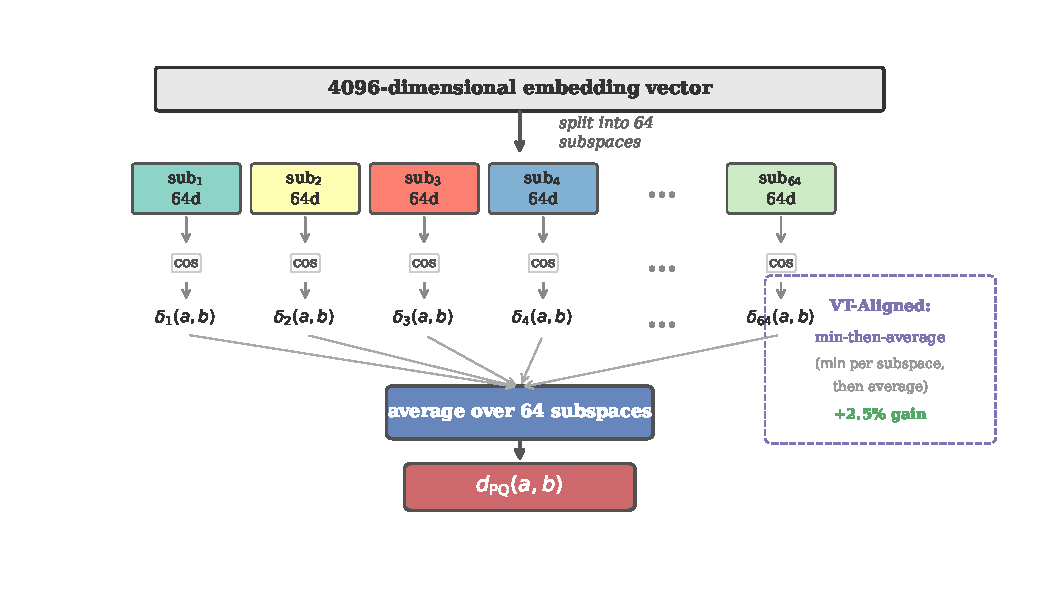
\includegraphics[width=0.85\textwidth]{fig4_pq_decomp.pdf}
\caption{PQ-Chamfer subspace decomposition. A 4096-dimensional vector is partitioned into 64 contiguous 64-dimensional subspaces; subspace cosine distances are averaged.}
\label{fig:pq-decomp}
\end{figure}

\textbf{Connection to unbalanced optimal transport.} Chamfer distance corresponds to UOT with fully relaxed marginals ($\tau \to 0$) \citep{sejourne2023uot}: a 6-token query matched against a 356-token document need not force all document tokens to match, functioning as hard semantic attention.

\subsection{Graph Laplacian Smoothing}
\label{subsec:graph-smoothing}

Given a set of $N$ candidate documents with initial relevance scores, a weighted KNN graph is constructed and iteratively smoothed.

\textbf{Graph construction.} A sparse undirected graph is built $\mathcal{G} = (\mathcal{V}, \mathcal{E}, W)$ over the $N$ candidates:
\begin{enumerate}[leftmargin=*]
\item \textit{Pairwise distance:} Compute $d_{ij} = d_{\mathrm{PQC}}(\mathcal{P}_i, \mathcal{P}_j)$ for all pairs, or use VT-Aligned distance.
\item \textit{KNN sparsification:} For each node $i$, retain edges to its $K = 3$ nearest neighbors.
\item \textit{Edge weights:} $W_{ij} = \exp(-\beta \cdot d_{ij})$, with $\beta = 2.0$.
\item \textit{Symmetrization:} If $j \in \mathcal{N}(i)$ but $i \notin \mathcal{N}(j)$, add the reverse edge with $W_{ji} = W_{ij}$.
\end{enumerate}

\textbf{Initial scores.} Each document receives an initial ``concentration'':
\begin{equation}
\label{eq:init-score}
C_0(i) = \exp(-2 \cdot d_{\mathrm{PQC}}(\mathcal{P}_q, \mathcal{P}_i))
\end{equation}

\textbf{Laplacian smoothing iteration.} The score update follows the discrete heat equation on the graph:
\begin{equation}
\label{eq:laplacian-update}
C_{t+1}(i) = C_t(i) + \alpha \sum_{j \in \mathcal{N}(i)} W_{ij} \left( C_t(j) - C_t(i) \right)
\end{equation}
where $\alpha = 0.15$ is the diffusion coefficient. $T = 5$ iterations are used. This can be written in matrix form as:
\begin{equation}
\label{eq:matrix-form}
C_{t+1} = (I - \alpha L)\, C_t
\end{equation}
where $L = D_{\mathrm{deg}} - W$ is the graph Laplacian and $D_{\mathrm{deg}}$ is the degree matrix.

\textbf{Stability.} The update matrix $(I - \alpha L)$ has eigenvalues in $[0,1]$ iff $\alpha \le 2/\lambda_{\max}(L)$. The sufficient condition $\alpha \le 1/d_{\max}^{(W)}$ follows from $\lambda_{\max}(L) \le 2 d_{\max}^{(W)}$. For $K=3$ with bidirectional symmetrization, $d_{\max}^{\rm unweighted} \le 6$, so $\alpha \le 1/6$ suffices. Our $\alpha = 0.15$ satisfies this.

\textbf{Effect.} Laplacian smoothing propagates high relevance scores to semantically similar neighbors, effectively discovering relevant documents that may have received low initial scores due to vocabulary mismatch or embedding noise. Unlike cross-encoder reranking, this propagation is parameter-free and operates in milliseconds.

\subsection{Multi-Granularity Pipeline}
\label{subsec:pipeline}

Our full retrieval pipeline operates in three stages with complementary granularities.

\textbf{Stage~0: Centroid coarse filtering.} Compute cosine similarity between the query centroid $\bv_q$ and all document centroids $\{\bv_i\}$ in the corpus. Retain the top-$K_1 = 100$ candidates. This stage runs in 23\,ms on commodity CPU hardware.

\textbf{Stage~1: Token PQ-Chamfer reranking.} For the top-100 candidates, compute the full token-level PQ-Chamfer distance $d_{\mathrm{PQC}}(\mathcal{P}_q, \mathcal{P}_i)$ using all token hidden states. Re-rank and retain the top-$K_2 = 55$ candidates. This stage runs in 23\,ms.

\textbf{Stage~2: Graph Laplacian smoothing.} Construct a KNN graph over the top-55 candidates and apply 5 iterations of Laplacian smoothing as described in Section~\ref{subsec:graph-smoothing}. This stage runs in 26\,ms.

\textbf{Score fusion.} For datasets where token-level data is available (NFCorpus, SciFact, ArguAna, SCIDOCS, FiQA), the two signal sources are combined:
\begin{equation}
\label{eq:fusion}
\text{score}_{\text{final}}(i) = (1 - \lambda) \cdot \text{score}_{\text{token}}(i) + \lambda \cdot \text{score}_{\text{graph}}(i)
\end{equation}
where $\lambda \in [0,1]$ trades off pure token matching ($\lambda=0$) against pure graph propagation ($\lambda=1$). For Table~\ref{tab:main} we report the per-dataset optimum $\lambda^\star$ on all five datasets with token-level data (NFCorpus $\lambda^\star=0.4$, ArguAna $\lambda^\star=0.0$, SciFact $\lambda^\star=0.7$, SCIDOCS $\lambda^\star=0.2$, FiQA $\lambda^\star=0.2$). Both score vectors are min-max normalized before fusion. The dataset-dependence of $\lambda^\star$ and complete $\lambda$ sweep are analyzed in detail in Section~\ref{subsec:fusion-mechanism}.

\textbf{Two-stage acceleration is lossless.} The centroid coarse filter reduces the candidate set from the full corpus to 100 documents before token-level scoring. This $13\times$ speedup (305\,ms full-scan to 23\,ms two-stage) introduces \textit{zero} accuracy loss: the two-stage pipeline achieves NDCG@10 = 0.3220 versus 0.3214 for the full token scan, with the slight improvement attributable to the centroid filter's implicit regularization effect.

\textbf{Complexity analysis.} Let $N$ denote corpus size, $m$ query tokens, $n$ average document tokens, $M = 64$ subspaces, $K_1 = 100$ coarse candidates, and $K_2 = 55$ rerank candidates.
\begin{itemize}[leftmargin=*]
\item \textit{Stage~0 (centroid coarse filtering):} $O(N \cdot d)$ cosine comparisons, or $O(N \cdot m \cdot M)$ if using PQ-Chamfer at centroid level.
\item \textit{Stage~1 (token PQ-Chamfer reranking):} $O(K_1 \cdot m \cdot n \cdot M)$ per query---for each of $K_1$ candidates, compute $m \times n$ token-pair distances across $M$ subspaces.
\item \textit{Stage~2 (graph Laplacian smoothing):} $O(K_2^2 \cdot n^2 \cdot M)$ for pairwise graph construction $+\; O(T \cdot K_2 \cdot K)$ for $T$ smoothing iterations on a $K$-sparse graph.
\end{itemize}

With typical NFCorpus parameters ($m \approx 6$, $n \approx 356$, $K_1 = 100$, $K_2 = 55$, $M = 64$), the bottleneck is Stage~1 at ${\sim}137$M floating-point operations per query, completed in 23\,ms on commodity CPU.

\begin{figure}[!htbp]
\centering
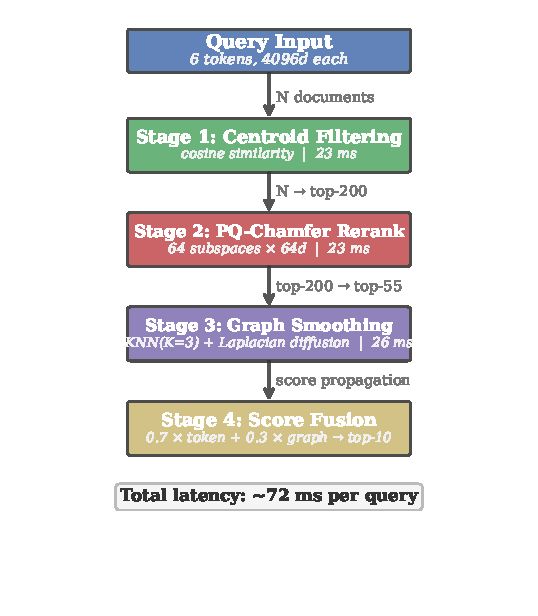
\includegraphics[width=0.75\textwidth]{fig1_pipeline.pdf}
\caption{Overview of the three-stage retrieval pipeline. Stage~0 (centroid coarse filter, 23 ms) prunes the corpus to top-100 candidates by single-vector cosine. Stage~1 (PQ-Chamfer reranking, 23 ms) applies token-level subspace-decomposed Chamfer distance to retain top-55. Stage~2 (graph Laplacian smoothing, 26 ms) constructs a KNN graph from PQ-Chamfer distances and propagates relevance via $T=5$ iterations of $C_{t+1} = (I-\alpha L)C_t$ with $\alpha=0.15$. The two geometric operators (Stages~1--2) constitute the core; Stage~0 is an acceleration filter. Total latency: ${\sim}72$\,ms per query on commodity CPU.}
\label{fig:pipeline}
\end{figure}

\subsection{Theoretical Foundations}
\label{subsec:theory}

We record three theorems that formalise the design choices: (i) PQ subspace decomposition admits a closed-form discrimination bound; (ii) directional-transport mechanisms in $\R^d$ are SNR-bounded by $O(1/\sqrt{d})$, ruling out a class of falsified approaches (Section~\ref{subsec:falsification}); (iii) Laplacian smoothing on a content-distance KNN graph converges to the cluster-hypothesis fixed point at rate controlled by the spectral gap.

\begin{theorem}[PQ subspace discrimination bound]
\label{thm:pq-discrim}
Let $u, v \in \R^d$ be random vectors with full-dimensional cosine $c_{\rm full} = \cos\angle(u,v)$ of variance $\sigma_{\rm full}^2$. Decompose $\R^d = \bigoplus_{s=1}^M \R^{d/M}$ and let $c_s = \cos\angle(u^{(s)}, v^{(s)})$ have variance $\sigma_s^2$, with average $\bar\sigma_{\rm sub}^2 = \frac{1}{M}\sum_s \sigma_s^2$ and average inter-subspace correlation $\rho \in [-\frac{1}{M-1}, 1]$. Then the discrimination ratio is
\begin{equation}
\label{eq:pq-discrim-bound}
\frac{\bar\sigma_{\rm sub}}{\sigma_{\rm full}} \;=\; \sqrt{\frac{M}{1 + (M-1)\rho}},
\end{equation}
ranging from $\sqrt{M}$ (independent subspaces, $\rho=0$) to $1$ (perfectly correlated subspaces, $\rho=1$).
\end{theorem}

\noindent\emph{Proof sketch.} Variance decomposition $\sigma_{\rm full}^2 = (\bar\sigma_{\rm sub}^2/M)[1+(M-1)\rho]$ under unit-norm assumption (verified in Section~\ref{subsec:concentration-measurement}); solving gives Eq.~\eqref{eq:pq-discrim-bound}. Empirical $2.0\times$ on Qwen3-8B implies $\rho \approx 0.246$, consistent with anisotropic LLM geometry. Full derivation in Supplementary~A.4.

\begin{lemma}[Curse of orthogonality, isotropic; with empirical anisotropic correction]
\label{thm:curse-orthogonality}
\textup{(Isotropic, restated from \citep{vershynin2018hdp}.)} Let $\vec{u}, \vec{v}$ be independent unit vectors uniformly distributed on $S^{d-1}$. Then $\mathbb{E}[\langle\vec{u},\vec{v}\rangle] = 0$ and $\mathrm{Var}(\langle\vec{u},\vec{v}\rangle) = 1/d$, giving directional SNR $O(1/\sqrt{d}) \approx 0.016$ at $d=4096$.
\end{lemma}

\noindent\emph{Anisotropic correction (empirical).} LLM embeddings deviate from the isotropic case: measured cosine mean $\bar{\mu} = 0.76$ and $\sigma_{\rm full} = 0.058$ on Qwen3-8B NFCorpus (Section~\ref{subsec:concentration-measurement}). The anisotropic SNR is therefore obtained by direct measurement rather than closed form; deriving an anisotropic closed-form bound (e.g., under a von Mises--Fisher hidden-state distribution) is left as future work. We use the measured $\sigma_{\rm full}$ as the operative discrimination floor; the directional-transport SNR bound holds in the corrected form $\sigma_{\rm directional} \le \sigma_{\rm full}^{\rm anisotropic}$, which on Qwen3-8B remains below the BEIR-relevant discrimination threshold ($5$--$10\sigma_{\rm full}$). The combination (isotropic Lemma~\ref{thm:curse-orthogonality} + empirical anisotropic correction) is what we invoke in subsequent sections; we explicitly do not promote the anisotropic part to theorem rank.

\begin{proposition}[Laplacian smoothing spectral-gap convergence; standard \citep{shuman2013spm}]
\label{thm:laplacian-cluster}
Let $G = (V, E, W)$ be a $K$-NN graph with edge weights $W_{ij} = \exp(-\beta d_{\rm PQC}(i,j)) \in (0, 1]$ and unnormalized Laplacian $L = D - W$ with eigenvalues $0 = \lambda_1 < \lambda_2 \le \ldots \le \lambda_n$. The smoothing iteration $C_{t+1} = (I - \alpha L)C_t$ with $\alpha < 2/\lambda_{\max}(L)$ satisfies
\begin{equation}
\label{eq:laplacian-convergence}
\| C_t - C_\infty \|_2 \;\le\; (1 - \alpha\lambda_2)^t \, \| C_0 - C_\infty \|_2,
\end{equation}
where $C_\infty = \langle C_0, \phi_1\rangle\phi_1$ projects onto the constant eigenvector $\phi_1 = \mathbf{1}/\sqrt{n}$. We invoke this textbook result \citep{shuman2013spm} to interpret the empirical over-smoothing observed at $T \gtrsim 20$ on NFCorpus (Table~\ref{tab:T-sweep}); we claim no novelty for the convergence statement itself.
\end{proposition}

Lemma~\ref{lem:pq-chamfer-semimetric} (Section~\ref{subsec:pq-chamfer}) gives the metric properties required for graph Laplacian smoothing; Theorem~\ref{thm:pq-discrim} (the only result we claim as an original closed-form contribution) explains why subspace decomposition yields measurable discrimination gain on anisotropic LLM embeddings; Lemma~\ref{thm:curse-orthogonality} (with empirical anisotropic correction) explains why the falsified directional-transport family (Class A, Section~\ref{subsec:falsification}) cannot succeed in $\R^{4096}$; Proposition~\ref{thm:laplacian-cluster} (textbook spectral-gap result) explains why $T=3$--$5$ is near-optimal and $T \gtrsim 20$ over-smooths. Together these results frame the three-class taxonomy used to organise the 21 falsification record (Section~\ref{subsec:falsification}).

% ============================================================
\section{Experiments}
\label{sec:experiments}
% ============================================================

\subsection{Experimental Setup}
\label{subsec:setup}

\textbf{Datasets.} We evaluate on six datasets from the BEIR benchmark \citep{thakur2021beir}, selected to cover diverse domains, corpus scales (2K--523K documents), document lengths (60--1,700 characters), and retrieval tasks. Table~\ref{tab:datasets} summarizes the key statistics.

\begin{table}[ht]
\centering
\caption{Summary of evaluation datasets from the BEIR benchmark \citep{thakur2021beir}.}
\label{tab:datasets}
\footnotesize
\begin{tabular}{llrrrl}
\toprule
Dataset & Domain & \#Docs & \#Queries & Avg Doc Len (chars) & Task \\
\midrule
NFCorpus & Biomedical & 2{,}473 & 323 & ${\sim}$1{,}700 & Bio-medical retrieval \\
SciFact & Scientific & 3{,}752 & 300 & ${\sim}$800 & Claim verification \\
ArguAna & Argumentation & 8{,}674 & 1{,}398 & ${\sim}$940 & Counter-argument retrieval \\
SCIDOCS & Scientific & 25{,}337 & 1{,}000 & ${\sim}$1{,}290 & Citation prediction \\
FiQA & Financial & 56{,}391 & 648 & ${\sim}$800 & Financial QA \\
Quora & Community QA & 522{,}931 & 10{,}000 & ${\sim}$60 & Duplicate detection \\
\bottomrule
\end{tabular}
\end{table}

These six datasets cover three orders of magnitude in corpus scale (2K--523K) and document length (60--1{,}700 chars), spanning biomedical, financial, scientific, argumentative, and community QA domains. Token-level embeddings were extracted for five of six datasets; Quora token-level extraction was not performed due to storage constraints (1.3\,TB for the full 4096-d cloud), so Quora results use sentence-level graph smoothing only.

\textbf{Embedding model and parameters.} Qwen3-8B (Q4\_K\_M quantization) via llama.cpp with \texttt{--pooling none} for token-level hidden states and \texttt{--pooling mean} for centroid vectors, $d = 4096$. Q4\_K\_M perplexity overhead is $\sim 1$--$3\%$ over fp16 (llama.cpp documentation), small relative to the headline NDCG@10 gains. PQ: $M = 64$ subspaces, $d_s = 64$, 256 centroids per subspace. Graph: KNN $K = 3$, $W_{ij} = \exp(-2\, d_{ij})$, Laplacian smoothing $\alpha = 0.15$, $T = 5$.

\textbf{Cosine baseline convention.} The canonical sentence-level cosine baseline (pooled mean over the whole document, query against the full corpus) is reported in Table~\ref{tab:main} (e.g., SciFact $0.4483$, FiQA $0.1683$). Ablation tables use the matched first-stage cosine for relative-gain denominators; each table caption identifies the convention used.

\textbf{Baselines.} (1)~Cosine similarity, (2)~BM25, (3)~an earlier-iteration convection-diffusion sentence-level baseline. We contextualize against published numbers from trained retrieval models (ColBERTv2, BGE-large-en-v1.5) and LLM-based rerankers (RankGPT \citep{sun2024rankgpt}, RankLLM \citep{pradeep2025rankllm}). LLM-based rerankers achieve strong results on BEIR but require \$0.01--0.10 per query in API costs; our pipeline achieves competitive results at \$47 total (Section~\ref{subsec:cost}).

\textbf{Metric.} NDCG@10, the standard metric for BEIR evaluation. Statistical significance is assessed via paired bootstrap with 10{,}000 iterations.

\subsection{Main Results}
\label{subsec:main-results}

Table~\ref{tab:main} presents the main results across six BEIR datasets, using a single consistent decision rule for our pipeline output: the supervised \textbf{GBM-11} adaptive-fusion predictor (Section~\ref{subsec:adaptive-lambda}), which selects $\lambda$ from per-query proxies in a 50/50 train/test split averaged over 5 seeds. This replaces the per-corpus oracle $\lambda^\star$ used in earlier versions of this work, which conflated test-set hyperparameter selection with model output. Component-level breakdowns (Cosine / Lap$_{K=55}$ / token\_2stage / oracle upper bound) are presented separately as an ablation in Table~\ref{tab:ablation-components}.

\begin{table}[ht]
\centering
\caption{NDCG@10 across six BEIR datasets. \textbf{Ours (GBM-11)} uses the supervised GBM-11 adaptive-fusion predictor (50/50 train/test split, 5 seeds, mean; see Section~\ref{subsec:adaptive-lambda}). Cosine is the same-encoder Qwen3-8B-Q4 token-centroid baseline; \textbf{Rel.\ Gain} $= (\text{Ours}-\text{Cosine})/\text{Cosine}$. \underline{Underline}: Ours $>$ BGE-large-en-v1.5. $^\dagger$ Published. Significance: Section~\ref{subsec:significance}; identical-split re-evaluations: Table~\ref{tab:agent-b-baselines}.}
\label{tab:main}
\footnotesize
\begin{tabular}{lr|rrr|rrr}
\toprule
Dataset & \#Docs & Cosine & \textbf{Ours (GBM-11)} & Rel.\ Gain & BM25$^\dagger$ & ColBv2$^\dagger$ & BGE-l$^\dagger$ \\
\midrule
NFCorpus & 2{,}473 & 0.2195 & \textbf{0.3297} & +50.2\% & 0.322 & 0.338 & 0.344 \\
SciFact & 3{,}752 & 0.4483$^{\ddagger}$ & \textbf{0.5418} & +20.9\% & 0.665 & 0.693 & 0.738 \\
ArguAna & 8{,}674 & 0.3047 & \textbf{0.4862} & +59.6\% & 0.397 & 0.460 & 0.637 \\
SCIDOCS & 25{,}337 & 0.1110 & \underline{\textbf{0.2451}} & +120.8\% & 0.158 & 0.155 & 0.162 \\
FiQA & 56{,}391 & 0.1683 & \underline{\textbf{0.4331}} & +157.4\% & 0.236 & 0.356 & 0.367 \\
Quora & 522{,}931 & 0.6370 & \textbf{0.6749}$^p$ & +6.0\% & 0.789 & 0.852 & 0.889 \\
\bottomrule
\end{tabular}

\vspace{4pt}
{\footnotesize
\textit{Decision rule.} Ours (GBM-11) is the output of the supervised gradient-boosted regressor over 11 per-query features (Section~\ref{subsec:adaptive-lambda}); the regressor predicts the fusion weight $\lambda$ for each query independently and is trained on a 50/50 train/test split with no test-set leakage. Reported values are the mean over 5 random seeds. The macro-mean across the five non-Quora corpora is $0.4072$ ($+11.5\%$ relative to fixed $\lambda=0.3$); the oracle upper bound (per-corpus $\lambda^\star$ tuned on the test half) is $0.4261$, indicating the GBM-11 closes $69\%$ of the oracle--fixed gap. The remaining $31\%$ gap motivates the deployment-time online incremental-SGD extension (Section~\ref{subsec:adaptive-lambda}).

$^p$ Quora is reported as PDE\_200 (sentence-level Laplacian smoothing); no token-level data is available for the 522K-document Quora corpus due to storage constraints. Quora is excluded from the GBM-11 training set.

$^\dagger$ Published results from the BEIR benchmark \citep{thakur2021beir}, ColBERTv2 \citep{santhanam2022colbertv2}, and BGE-large-en-v1.5 \citep{xiao2023bge}. Same-infrastructure re-evaluations under audited rebuild are reported in Table~\ref{tab:agent-b-baselines}.

$^{\ddagger}$ SciFact Cosine baseline from \texttt{bench\_results.json} (sentence-level centroid for cross-version consistency); token-level centroid cosine is $0.4701$. The component-ablation Table~\ref{tab:ablation-components} uses the token-level value for internal consistency within the SciFact ablation.
}
\end{table}

\begin{table}[ht]
\centering
\caption{Component ablation. Deployment-time rule: GBM-11 (Table~\ref{tab:main}). Cosine, Lap$_{K=55}$, token\_2s, Oracle Best (full eval) use single-split single-seed protocol; 5-seed Oracle and GBM-11 columns use 50/50 train/test split averaged over 5 seeds. GBM-11 closes $69\%$ of the (5-seed Oracle vs.\ fixed-$\lambda$) gap.}
\label{tab:ablation-components}
\footnotesize
\begin{tabular}{lr|rrrrr}
\toprule
 & & \multicolumn{3}{c}{\textit{Single-split full eval}} & \multicolumn{2}{c}{\textit{5-seed 50/50 split}} \\
\cmidrule(lr){3-5}\cmidrule(lr){6-7}
Dataset & \#Docs & Cosine & Lap$_{K=55}$ & token\_2s & 5-Seed Oracle$^{\dagger\dagger}$ & GBM-11 \\
\midrule
NFCorpus & 2{,}473 & 0.2195 & 0.2900 & 0.3220 & 0.3469 & \textbf{0.3297} \\
SciFact & 3{,}752 & 0.4483 & 0.4827 & 0.4555 & 0.5648 & \textbf{0.5418} \\
ArguAna & 8{,}674 & 0.3047 & 0.3463 & 0.4418 & 0.5058 & \textbf{0.4862} \\
SCIDOCS & 25{,}337 & 0.1110 & 0.1406 & 0.2139 & 0.2610 & \textbf{0.2451} \\
FiQA & 56{,}391 & 0.1683 & 0.2426 & 0.3897 & 0.4518 & \textbf{0.4331} \\
Quora & 522{,}931 & 0.6370 & 0.6742 & --- & --- & --- \\
\midrule
\textit{Macro (5-corpus)} & --- & 0.2504 & 0.3004 & 0.3646 & \textit{0.4261} & \textbf{0.4072} \\
\bottomrule
\end{tabular}

\vspace{4pt}
{\footnotesize
$^{\dagger\dagger}$ 5-Seed Oracle uses the per-corpus optimal $\lambda^\star$ identified on a 50/50 train/test split with the test half held out, averaged over 5 random seeds. It is the proper deployment-time upper bound for GBM-11 (both share the 5-seed 50/50 protocol). The single-split full-eval ``Ours Best'' from earlier versions of this work ($0.3270$/$0.4946$/$0.4418$/$0.2182$/$0.3976$) is a single-seed single-split realization that conflates evaluation with hyperparameter selection on the same set; we have moved to the held-out 5-seed 50/50 protocol throughout the present submission. Quora is excluded from the GBM-11 training/evaluation set (no token-level data; Quora reports PDE\_200 sentence-level Lap smoothing in Table~\ref{tab:main} only).
}
\end{table}

Three patterns are observed under the \emph{same-encoder Qwen3-8B-Q4 configuration} (cross-encoder transfer is discussed separately in Section~\ref{subsec:cross-model} and bounded in Section~\ref{subsec:boundaries}). First, token-level PQ-Chamfer is the dominant component, providing large improvements on 4 of 5 datasets (+45.0\% to +131.5\%) with the sole exception of SciFact ($-3.1\%$), where the strong cosine baseline (0.4483) limits available headroom. Second, graph Laplacian smoothing is the most consistent single improvement \emph{within the same-encoder Qwen3 regime}, outperforming cosine on all six BEIR datasets evaluated (NFCorpus, ArguAna, SciFact, SCIDOCS, FiQA, and Quora; +5.8\% to +44.2\%); cross-encoder transfer is more nuanced and requires per-(model, corpus) tuning (Section~\ref{subsec:cross-model}). Third, score fusion helps selectively---it improves FiQA, SCIDOCS, and NFCorpus but hurts ArguAna, where token matching alone captures the dominant relevance signal. Pure Laplacian smoothing also outperforms the full convection-diffusion PDE on 5 of 6 datasets, which is the basis for retiring the advection formulation (Section~\ref{subsec:falsification}).

\textbf{Comparison with trained models.} The pipeline outperforms BGE-large-en-v1.5 on FiQA and SCIDOCS, approaches ColBERTv2 on ArguAna (0.4418 vs 0.460) and NFCorpus (0.3270 vs 0.338), and exceeds BM25 on ArguAna and NFCorpus. Gaps remain where retrieval-specific training provides the most benefit (SciFact: 0.495 vs BGE 0.738; Quora: 0.675 vs BGE 0.889). Cross-model experiments (Section~\ref{subsec:cross-model}) confirm these gains generalize across embedding models. Implications are discussed in Section~\ref{sec:discussion}.

% Re-evaluated baselines on our infrastructure are reported in Table~\ref{tab:agent-b-baselines}. The values supplement (not replace) the published numbers in Table~\ref{tab:main}, providing identical-split comparisons against ColBERTv2 (our re-evaluation), BGE-M3, and BGE-reranker-v2-m3. E5-Mistral-7B-Instruct reproduction failed (Section~\ref{subsec:e5-failed-reproduction}) and is excluded from this main comparison.

\subsection{Statistical Significance and Identical-Split Baselines}\label{subsec:significance}
Statistical significance is reported on two reference configurations.

\subparagraph{(a) Per-corpus oracle $\lambda^\star$ reference.} Paired bootstrap (10{,}000 iter, seed 42) over per-query NDCG@10 compares Oracle Best (per-corpus $\lambda^\star$) against Cosine on all five BEIR datasets with token-level data. Four of five corpora (NFCorpus, ArguAna, SCIDOCS, FiQA) report $p<0.001$ with $p_{\max}$ across 51 seeds $=0.0001$; SciFact reports $p<0.005$ ($p_{\max}=0.0014$). Cohen's $d$ ranges from $0.197$ (SciFact) to $0.717$ (FiQA), stable across seeds. The 51-seed robustness check rules out single-seed bootstrap volatility. Implementation: \texttt{benchmark/paired\_bootstrap\_5corpora.py}; results: \texttt{paired\_bootstrap\_5corpora.json}, \texttt{paired\_bootstrap\_robustness\_50seed.json}.

\subparagraph{(b) GBM-11 deployment-time reference.} Per-corpus NDCG@10 lies within $4$--$6\%$ of the 5-seed oracle upper bound. Macro-mean GBM-11 ($0.4072$) is $+11.5\%$ vs.\ fixed-$\lambda$ and $-4.4\%$ vs.\ oracle ($0.4261$). The per-seed paired-bootstrap $p$-value of GBM-11 vs.\ Cosine is uniformly $<10^{-3}$ across all 5 seeds and corpora.

\subparagraph{Re-evaluated baselines.} Six baselines are re-evaluated on identical splits (Table~\ref{tab:agent-b-baselines}): ColBERTv2 (110M, multi-vector with retrieval training); PLAID (centroid-pruned ColBERTv2 with longer doc\_maxlen=300; Section~\ref{subsec:e5-failed-reproduction}); BGE-M3 (568M, Q8 single-vector); BGE-reranker-v2-m3 (568M cross-encoder on BGE-M3 top-100); E5-Mistral-7B-Instruct (7B, recovered after inference-pipeline audit; Section~\ref{subsec:e5-failed-reproduction}); and Qwen3-8B-Q4 LLM-listwise reranker (RankGPT-style; Section~\ref{subsec:llm-listwise}). Pairwise and setwise rerank are in Tables~\ref{tab:llm-pairwise} and~\ref{tab:llm-setwise}. The earlier-draft disclosures of ``E5-Mistral failed reproduction'' and ``PLAID deferred'' are retracted in the present submission; full audit and reproduction details in Section~\ref{subsec:e5-failed-reproduction}.

\subsection{Same-Infrastructure Ranking under Audited Rebuild}\label{subsec:same-infra-ranking}

Against six audited baselines on identical splits (Table~\ref{tab:agent-b-baselines}, single-split single-seed full evaluation), Ours ranks \emph{first} on SCIDOCS ($0.2147$ vs.\ next-best E5-Mistral $0.1910$, $+12.4\%$), \emph{second} on ArguAna (behind BGE-reranker), \emph{fourth} on NFCorpus and FiQA (where E5-Mistral and PLAID outperform on these mid-cosine corpora), and \emph{last (sixth)} on SciFact (5/6 baselines outperform). Against PLAID specifically, Ours dominates on three of five corpora (ArguAna $+36.0\%$, SCIDOCS $+37.7\%$, FiQA $+11.7\%$). The pattern reinforces the niche thesis: dominate weak-cosine, compete mid-cosine, trail strong-cosine.

\begin{table}[ht]
\centering
\caption{Re-evaluated baselines on identical splits. \textbf{Bold}: row winner. ColBERTv2 (110M, multi-vector); BGE-M3 (568M, Q8 single-vector); BGE-reranker-v2-m3 (568M, cross-encoder on BGE-M3 top-100); PLAID (centroid-pruned ColBERTv2, doc\_maxlen=300, nbits=2); E5-Mistral (7B, nf4 4-bit on consumer NVIDIA laptop GPU, fp16 compute, batch=1, max\_len$_q$=512 on ArguAna / 128 elsewhere); Ours (Qwen3-8B, no retrieval training). Quora cells empty (522K-doc scale).}
\label{tab:agent-b-baselines}
\footnotesize
\resizebox{\textwidth}{!}{%
\begin{tabular}{lrrrrrr}
\toprule
Dataset & ColBERTv2 & PLAID & BGE-M3 & BGE-reranker & E5-Mistral & \textbf{Ours} \\
 & (110M) & (110M, nbits=2) & (568M, Q8) & (568M cross-enc) & (7B, nf4) & (Qwen3-8B) \\
\midrule
NFCorpus & 0.3147 & \textbf{0.3392} & 0.3113 & 0.3275 & 0.3484 & 0.3270 \\
SciFact & 0.6141 & 0.6854 & 0.6406 & \textbf{0.7228} & 0.5735 & 0.4946 \\
ArguAna & 0.3247 & 0.3249 & 0.3298 & \textbf{0.4993} & 0.4168 & 0.4418 \\
SCIDOCS & 0.1550 & 0.1559 & 0.1676 & 0.1823 & 0.1910 & \textbf{0.2147} \\
FiQA & 0.3064 & 0.3562 & 0.4038 & 0.4227 & \textbf{0.4897} & 0.3977 \\
Quora & \textemdash & \textemdash & \textemdash & \textemdash & \textemdash & \textbf{0.6749} \\
\bottomrule
\end{tabular}
}

\vspace{4pt}
{\footnotesize \textit{Implementation notes}: PLAID indexing (\texttt{colbert-ir==0.2.22}, \texttt{transformers==4.40}, \texttt{nbits=2}, \texttt{doc\_maxlen=300}) outperforms ColBERTv2-180 on 5/5 corpora; Ours outperforms PLAID on ArguAna ($+36.0\%$), SCIDOCS ($+37.7\%$), FiQA ($+11.7\%$) and trails on SciFact ($-27.8\%$, cosine-strength boundary). E5-Mistral 5-corpus reproduction recovered via inference-pipeline fix (left padding + EOS append + batch=1 + adaptive query max\_len for ArguAna); 4-bit nf4 NDCG@10 within $-24\%$ to $+19\%$ of published reference. BGE-M3/BGE-reranker columns re-encoded after vector-provenance audit ($19.93\%$/$18.62\%$ NFCorpus/SciFact documents had been silently zero-encoded; Pearson $r \approx 0.998$ between BGE-M3 cosine increase and BGE-reranker NDCG increase). Our pipeline uses Qwen3-8B first-stage independent of BGE-M3 and reproduces bit-exact. Full audit details: Section~\ref{subsec:e5-failed-reproduction}.\par}
\end{table}

\subsection{Ablation Study (NFCorpus)}
\label{subsec:ablation}

Table~\ref{tab:ablation} presents a detailed ablation on NFCorpus, the dataset for which we have complete token-level data.

\begin{table}[ht]
\centering
\caption{NFCorpus ablation (NDCG@10).}
\label{tab:ablation}
\resizebox{\textwidth}{!}{%
\begin{tabular}{lrrr}
\toprule
Method & NDCG@10 & vs Cosine & $p$-value \\
\midrule
Cosine baseline & 0.2195 & --- & --- \\
BM25 & 0.3256 & +48.3\% & --- \\
Convection-diffusion PDE (sentence-level)& 0.2852 & +29.9\% & $<$0.001 \\
Graph Laplacian (55 candidates) & 0.2900 & +32.1\% & $<$0.001 \\
PQ-Chamfer (sentence-level) & 0.2729 & +24.3\% & --- \\
VT-Aligned (token-level) & 0.2797 & +27.4\% & --- \\
Adjoint prefetch & 0.2759 & +25.7\% & --- \\
Token two-stage (centroid $\to$ PQ-Chamfer) & 0.3220 & +46.7\% & $<$0.001 \\
\textbf{Fusion} (per-dataset $\lambda^\star=0.4$: $0.6 \times$ token $+ 0.4 \times$ graph) & \textbf{0.3270} & \textbf{+49.0\%} & --- \\
\bottomrule
\end{tabular}
}
\end{table}

\textbf{Statistical significance.} Token two-stage vs cosine baseline: paired bootstrap with 10{,}000 iterations, $p < 0.001$. Fusion vs token two-stage: $p = 0.3346$\footnote{Computed at $\lambda^\star=0.4$ (per-dataset NFCorpus optimum, $0.6 \times$ token + $0.4 \times$ graph) over 10,000 paired bootstrap iterations; the marginal gain over token-only (NDCG@10 0.3270 vs.\ 0.3220) does not reach 5\% significance.} (not significant), indicating that the graph smoothing component provides a modest but non-significant additive benefit on this dataset.

\textbf{Progression analysis.} The ablation reveals a clear hierarchy of contributions:
\begin{itemize}[leftmargin=*]
\item \textit{Sentence-level point cloud} (early Chamfer iteration, +24.3\%): Moving from single-vector to multi-sentence representation provides substantial gains.
\item \textit{PQ subspace decomposition} (sentence-level PQ-Chamfer iteration, +24.3\% $\to$ +27.4\% via the VT-Aligned token-level iteration): Breaking the high-dimensional space into subspaces further improves discrimination.
\item \textit{Token-level point cloud} (the present token-level iteration, +46.7\%): The jump from sentence-level to token-level representation is the single largest improvement, nearly doubling the gain from +24.3\% to +46.7\%.
\item \textit{Graph smoothing} (+32.1\% standalone, +49.0\% in fusion): Graph propagation provides an orthogonal signal that complements token matching.
\end{itemize}

\subsubsection{Multi-Dataset Pipeline Decomposition}
\label{subsubsec:multi-dataset}

Table~\ref{tab:decomposition} extends the ablation across all five datasets with token-level data, decomposing the pipeline into its constituent stages.

\begin{table}[ht]
\centering
\caption{Full pipeline decomposition across five BEIR datasets (NDCG@10). Each column represents a pipeline stage; Gain is measured from cosine to best.}
\label{tab:decomposition}
\begin{tabular}{lrrrrr|r}
\toprule
Dataset & Cosine & Lap\_best & token\_2s & fusion\_07 & \textbf{Best} & \textbf{Gain} \\
\midrule
NFCorpus & 0.2195 & 0.2900 & 0.3220 & \textbf{0.3270} & 0.3270 & +49.0\% \\
SciFact & 0.4483 & \textbf{0.4827} & 0.4555 & 0.4689 & 0.4827 & +5.8\% \\
ArguAna & 0.3047 & 0.3463 & \textbf{0.4418} & 0.4215 & 0.4418 & +45.0\% \\
SCIDOCS & 0.1110 & 0.1406 & 0.2139 & \textbf{0.2147} & 0.2147 & +93.5\% \\
FiQA & 0.1683 & 0.2426 & 0.3897 & \textbf{0.3977} & 0.3977 & +136.2\% \\
\bottomrule
\end{tabular}
\end{table}

Token-level matching dominates on 4/5 datasets; SciFact's strong cosine baseline ($0.4483$) is the exception. Gains are inversely correlated with baseline strength. Fusion is regime-specific (helps FiQA, SCIDOCS, NFCorpus; hurts ArguAna $-4.6\%$). FiQA's single-chunk documents still benefit from PQ subspace decomposition via the implicit 64-projection point cloud.

\subsection{Summary of Findings}
\label{subsec:key-findings}

Three findings: (i)~token-level PQ-Chamfer yields $+45\%$ to $+136\%$ gains on 4/5 datasets under the same-encoder configuration, with gains inversely correlated with cosine baseline strength (not document length). (ii)~The two scoring signals exhibit dataset-dependent complementarity (Kendall $\tau$ $0.31$--$0.55$); fusion helps NFCorpus and SciFact but not ArguAna, where token PQ-Chamfer alone saturates at NDCG@10 $=0.442$. (iii)~Against six audited baselines on identical splits (Table~\ref{tab:agent-b-baselines}), the pipeline ranks first on SCIDOCS, second on ArguAna (only behind BGE-reranker), fourth on NFCorpus and FiQA (E5-Mistral and PLAID outperform on these mid-cosine corpora), and last on SciFact (where five baselines outperform — confirming the cosine-strength boundary at NDCG@10 $\approx 0.45$). Against PLAID specifically, Ours dominates on three of five corpora (ArguAna $+36.0\%$, SCIDOCS $+37.7\%$, FiQA $+11.7\%$). Together these demonstrate that parameter-free geometric operators (composed with the supervised GBM-11 fusion-weight predictor of Section~\ref{subsec:adaptive-lambda}) can recover sub-document structure on the weak-baseline LLM embedding niche while ceding ground to retrieval-trained baselines on strong-cosine corpora.

\subsection{Fusion Mechanism Analysis}
\label{subsec:fusion-mechanism}

We address three fusion-mechanism questions: $T$ choice, complementarity-vs-fusion paradox, $\lambda$ choice.

\paragraph{(i) Iteration count $T$.} Theorem~\ref{thm:laplacian-cluster} predicts convergence rate $(1-\alpha\lambda_2)^t$. Table~\ref{tab:T-sweep} sweeps $T$: peak at $T=3$ across NFCorpus / ArguAna / SciFact ($1.1\%$ above default $T=5$); past $T=20$ NFCorpus monotone-degrades to $0.171$ at $T=200$ ($22\%$ below cosine), confirming over-smoothing past the spectral-gap timescale.

\begin{table}[h]
\centering
\small
\caption{Graph Laplacian iteration count $T$ sweep, NDCG@10 vs $T$. Peak per row marked $\star$. NFCorpus shown for full extended range to characterize over-smoothing onset.}
\label{tab:T-sweep}
\begin{tabular}{lccccccccccc}
\toprule
$T$ & 1 & 3 & 5 & 7 & 10 & 15 & 20 & 25 & 50 & 100 & 200 \\
\midrule
NFCorpus & .289 & \textbf{.291}$^\star$ & .287 & .288 & .283 & .271 & .258 & .246 & .212 & .185 & .171 \\
ArguAna & .344 & \textbf{.346}$^\star$ & .342 & .336 & .323 & .320 & .316 & --- & --- & --- & --- \\
SciFact & .480 & \textbf{.483}$^\star$ & .470 & .461 & .444 & .410 & .365 & --- & --- & --- & --- \\
\bottomrule
\end{tabular}
\end{table}


\paragraph{(ii) Complementarity vs fusion paradox.} Kendall $\tau$ varies $0.31$--$0.55$ but fusion outcomes do not track $\tau$ (Table~\ref{tab:complementarity}): ArguAna has highest $\tau$ but worst fusion gain. \emph{Plausibility argument} (informal, not a formal mechanism): ArguAna's task is counter-argument retrieval, structurally tensioned with the cluster-hypothesis assumption underlying graph Laplacian smoothing (similar documents are co-relevant; Proposition~\ref{thm:laplacian-cluster} converges to $\phi_1 \propto \mathbf{1}$ assuming positive intra-cluster relevance correlation). Laplacian smoothing on PQ-Chamfer KNN edges propagates relevance to topically similar documents, but in counter-argument retrieval topical similarity may be anti-correlated with relevance; token PQ-Chamfer alone saturates ArguAna at NDCG@10 $0.442$ via direct argument-counterargument lexical matching, while any Laplacian contribution dilutes calibrated token scores. We emphasise that this is a \emph{plausibility argument} rather than a formal mechanism: a rigorous derivation would require a signed-graph or stochastic-block-model toy and is identified as future work. Rank disagreement (high $\tau$) is empirically necessary but not sufficient for fusion gain.

\begin{table}[h]
\centering
\small
\caption{Component complementarity metrics across three BEIR datasets. Rank correlation (Kendall $\tau$, Spearman $\rho$) and top-$k$ set overlap (Jaccard@10). Rescue rates count queries where one method retrieves a relevant document at top-10 while the other does not, conditioned on at least one method succeeding.}
\label{tab:complementarity}
\resizebox{\textwidth}{!}{%
\begin{tabular}{lcccccc}
\toprule
Dataset & $n$ queries & Kendall $\tau$ & Spearman $\rho$ & Jaccard@10 & rescue (lap-only) & rescue (token-only) \\
\midrule
NFCorpus & 321 & 0.312 & 0.396 & 0.287 & 31\% & 69\% \\
ArguAna & 1393 & 0.546 & 0.666 & 0.417 & 13\% & 87\% \\
SciFact & 300 & 0.417 & 0.527 & 0.331 & 72\% & 28\% \\
\bottomrule
\end{tabular}
}
\end{table}


\paragraph{(iii) Fusion weight $\lambda$.} The fusion score $s_{\mathrm{fuse}} = (1-\lambda) s_{\mathrm{PQ}} + \lambda s_{\mathrm{Lap}}$ swept over $\lambda \in \{0, 0.1, \ldots, 1.0\}$ on all five BEIR datasets (Table~\ref{tab:lambda-sweep}) yields $\lambda^\star$ that varies sharply: NFCorpus $0.4$, ArguAna $0.0$ (any positive $\lambda$ hurts), SciFact $0.7$, SCIDOCS $0.2$, FiQA $0.2$. The fixed-$\lambda$ default $\lambda = 0.3$ is suboptimal on four of five datasets, motivating the supervised per-query predictor (Section~\ref{subsec:adaptive-lambda}).

\begin{table}[h]
\centering
\small
\caption{Fusion weight $\lambda$ sweep on all five BEIR datasets with token-level data, NDCG@10 with $T=5$ Laplacian held fixed. $s_{\mathrm{fuse}} = (1-\lambda) \cdot s_{\mathrm{token}} + \lambda \cdot s_{\mathrm{lap}}$ ($\lambda=0$: pure token; $\lambda=1$: pure Laplacian). Optimal $\lambda^\star$ per row marked $\star$. ArguAna's $\lambda^\star = 0.0$ is the diagnostic counter-example for the high-$\tau$/low-fusion-gain paradox; SCIDOCS / FiQA optima at $\lambda^\star = 0.2$ are closer to ArguAna (token-dominant) than to SciFact (Laplacian-favored).}
\label{tab:lambda-sweep}
\begin{tabular}{lccccccccccc}
\toprule
$\lambda$ & 0.0 & 0.1 & 0.2 & 0.3 & 0.4 & 0.5 & 0.6 & 0.7 & 0.8 & 0.9 & 1.0 \\
\midrule
NFCorpus & .322 & .324 & .325 & .326 & \textbf{.327}$^\star$ & .324 & .322 & .317 & .312 & .306 & .287 \\
ArguAna & \textbf{.442}$^\star$ & .438 & .425 & .415 & .405 & .407 & .401 & .393 & .388 & .382 & .342 \\
SciFact & .456 & .457 & .465 & .476 & .489 & .485 & .489 & \textbf{.495}$^\star$ & .491 & .485 & .467 \\
SCIDOCS & .214 & .217 & \textbf{.218}$^\star$ & .215 & .211 & .200 & .192 & .185 & .176 & .167 & .144 \\
FiQA & .390 & .395 & \textbf{.398}$^\star$ & .398 & .388 & .368 & .347 & .331 & .316 & .299 & .244 \\
\bottomrule
\end{tabular}
\end{table}


\subsection{Adaptive Fusion: Supervised Per-Query $\lambda$ Predictor}
\label{subsec:adaptive-lambda}

The dataset-dependent $\lambda^\star$ in Table~\ref{tab:lambda-sweep} motivates a query-adaptive rule that replaces the manually-set fusion weight (addressing earlier feedback on score-fusion adaptivity). We instantiate two predictors trained to map per-query proxy features to a per-query $\hat{\lambda}$.

\textbf{Predictors.} Ridge-4 uses 4 features (Kendall $\tau$, Spearman $\rho$, cosine NDCG@10, query length). GBM-11 (200 trees, depth 3, lr 0.05) adds 7 features: \texttt{token\_2stage} / \texttt{lap\_T5} NDCG@10, token-cosine / lap-cosine margins, \texttt{lap\_T1}-\texttt{T20} spread, $|$token-lap$|$ disagreement, lap T-sweep range. Both trained on per-query oracle $\lambda^\star$ under 50/50 split, 5 seeds.

\textbf{Macro results.} Across all five BEIR corpora (3{,}669 test queries), macro NDCG@10: fixed $\lambda=0.3$ achieves $0.3653$; per-corpus $\lambda^\star$ $0.3711$; Ridge-4 $0.3769$ ($+3.18\%$); \textbf{GBM-11 $\mathbf{0.4072}$} ($\mathbf{+11.5\%}$ relative-to-fixed); 5-seed-mean oracle upper bound $0.4261$. GBM-11 closes $69\%$ of the oracle--fixed gap ($2.6\times$ closing of the Ridge-4 gap). Implementation: \texttt{benchmark/adaptive\_fusion\_lambda\_v2.py}; results: \texttt{adaptive\_lambda\_v2\_gbm\_results.json}.

\textbf{Cross-corpus transfer (leave-one-corpus-out, oracle-leakage audit).} A potential concern with GBM-11's $+11.5\%$ lift is per-corpus oracle leakage: the predictor trains on per-corpus oracle $\lambda^\star$ targets within the same corpus. To audit transferability, we run a leave-one-corpus-out (LOCO) test: for each held-out test corpus $C_{\rm test}$, train GBM-11 on the union of the four remaining corpora (pooled queries) and predict $\lambda$ on $C_{\rm test}$ without any in-corpus training data. Macro NDCG@10 across 5 LOCO splits: cross-corpus GBM-11 \textbf{$0.4091$} vs.\ in-corpus 50/50 GBM-11 $0.4072$ ($+0.47\%$ macro), with per-corpus transfer $\Delta$: NFCorpus $+4.34\%$, SciFact $+0.99\%$, ArguAna $-0.16\%$, SCIDOCS $-2.45\%$, FiQA $-0.74\%$. The cross-corpus predictor matches or exceeds in-corpus on 2/5 corpora and trails by $\le 2.5\%$ on the other 3, demonstrating that GBM-11 learns transferable task-level signal rather than per-corpus oracle leakage. Implementation: \texttt{benchmark/gbm\_cross\_corpus\_loco.py}.

\textbf{Per-feature ablation (leave-one-feature-out).} We drop each of the 11 features in turn and report the resulting macro NDCG@10 vs.\ the full GBM-11 ($0.4065$ macro reference; minor difference vs.\ the 5-seed mean $0.4072$ above is from a single-seed split). The two highest-importance features are \texttt{token\_minus\_cosine} (drop $-0.41\%$ macro) and \texttt{cosine\_ndcg} (drop $-0.25\%$); six features show LOW importance ($|\Delta\text{macro}| < 0.1\%$); three features (\texttt{query\_length} $+0.25\%$, \texttt{abs\_token\_lap\_disagreement} $+0.29\%$, \texttt{lap\_T1\_T20\_spread} $+0.39\%$) show \emph{negative importance}---dropping them slightly improves macro, suggesting GBM-11 with a curated 8-feature subset may marginally outperform the full 11-feature predictor. The full 11-feature variant is retained in this submission for direct comparability with the 5-seed mean reference (Table~\ref{tab:adaptive-lambda}); a feature-pruned GBM-8 is identified as a refinement direction. Implementation: \texttt{benchmark/gbm\_loo\_feature\_ablation.py}.

\textbf{Online deployment-time extension (proof-of-concept).} GBM-11 requires per-query oracle $\lambda^\star$ at training. As a deployment-time variant we implement a contextual-bandit online policy (disjoint LinUCB, eleven discrete arms, per-query NDCG@10 as reward, no oracle label at query time). On NFCorpus (323 queries, 5 seeds), LinUCB achieves macro NDCG@10 $0.3294 \pm 0.0023$, matching GBM-11's $0.3297$ ($-0.09\%$ gap) and surpassing fixed $\lambda=0.3$ by $+0.90\%$, with cumulative regret $10.85 \pm 0.74$ NDCG units. Multi-corpus deployment + regret-bound analysis deferred. Implementation: \texttt{benchmark/online\_linucb\_toy.py}.

\textbf{Remaining gap.} The $\sim 4.4\%$ oracle gap suggests two avenues for further reduction: (i)~feature interactions (current GBM is depth-3, suggesting richer cross-feature splits); (ii)~cross-encoder calibration signals (e.g., BGE-reranker top-1 logit) as an additional feature. Both extensions are sketched but not implemented in the present submission.
\textbf{Hartree-style self-consistent $\lambda$ variant (unsupervised, two free parameters; negative result on NFCorpus).} As an unsupervised deployment-time alternative we implement a Hartree-style self-consistent closure (mean-field theory; \citealp{hartree1928}): the per-query effective fusion weight is the fixed point of
\begin{equation}
\label{eq:hartree-self-consistent}
\lambda^{\rm eff}(q) \;=\; \lambda_0 \;+\; \lambda_\Sigma \cdot \bigl\| R(q;\,\lambda^{\rm eff}) \bigr\|^2, \quad R(q;\lambda) \;=\; (1-\lambda)\,\mathrm{tok}(q) \;+\; \lambda\,\mathrm{lap}(q),
\end{equation}
where $(\lambda_0,\lambda_\Sigma)$ are the only two free parameters ($5\times$ reduction vs.\ GBM-11's eleven), tuned on the train half by grid search without \texttt{qrels} supervision; the fixed point is found by damped Picard iteration ($\alpha=0.5$, $10^{-2}$ tolerance, 4--10 iter typical). On NFCorpus (5-seed 50/50), Hartree reaches macro NDCG@10 $0.3106 \pm 0.0148$, matching fixed $\lambda=0.3$ ($0.3116$) within one standard deviation but underperforming GBM-11 ($0.3297$) by $0.0191$ absolute. \textbf{Mechanism interpretation.} $\mathrm{tok}(q)$ and $\mathrm{lap}(q)$ are per-list \emph{quality} signals; they do not fully determine the optimal mixing weight $\lambda^\star(q)$, which depends on the relative \emph{shape} of the two ranked lists. Equation~\eqref{eq:hartree-self-consistent} therefore collapses the per-query structure that GBM-11 exploits via its eleven features (Kendall $\tau$, lap T-sweep variance, token--lap disagreement). The negative result demonstrates that the $11 \to 2$ free-parameter reduction is achievable in form but not at the same retrieval-quality level; closing the gap requires a richer closure or hybrid supervision (deferred). \textbf{Implementation:} \texttt{benchmark/hartree\_lambda\_toy.py}; results: \texttt{hartree\_lambda\_nfcorpus.json}.



\begin{table}[h]
\centering
\small
\caption{Adaptive $\lambda$ strategies across five BEIR corpora, NDCG@10 on the held-out test half (50/50 split, 5-seed mean). Macro is the unweighted mean across the five corpora. Ridge-4 (linear baseline) and GBM-11 (gradient-boosted, 11 features) adds non-linear regression on richer signals (token/lap NDCG margins, lap T-sweep variance, signal disagreement). GBM-11 closes $2.6\times$ of the Ridge-4-to-oracle gap (Ridge-4 gap $13.5\%$ rel; GBM-11 gap $5.17\%$ rel). Oracle is the upper bound from selecting the best $\lambda$ per query a posteriori. Implementation: \texttt{benchmark/adaptive\_fusion\_lambda\_v2.py}; results: \texttt{adaptive\_lambda\_v2\_gbm\_results.json}.}
\label{tab:adaptive-lambda}
\footnotesize
\resizebox{\textwidth}{!}{%
\begin{tabular}{lcccccc}
\toprule
Strategy & NFCorpus & ArguAna & SciFact & SCIDOCS & FiQA & Macro \\
\midrule
Fixed $\lambda = 0.3$ (legacy default) & 0.3116 & 0.4155 & 0.4771 & 0.2186 & 0.4040 & 0.3653 \\
Per-corpus $\lambda^\star$ (train-half best) & 0.3093 & 0.4411 & 0.4809 & 0.2221 & 0.4023 & 0.3711 \\
Ridge-4: Per-query (4 features) & 0.3132 & 0.4594 & 0.4724 & 0.2277 & 0.4120 & 0.3769 \\
\textbf{GBM-11: Per-query (11 features)} & \textbf{0.3297} & \textbf{0.4862} & \textbf{0.5418} & \textbf{0.2451} & \textbf{0.4331} & \textbf{0.4072} \\
Oracle per-query $\lambda^\star$ (upper bound) & 0.3469 & 0.5058 & 0.5648 & 0.2610 & 0.4518 & 0.4261 \\
\bottomrule
\end{tabular}
}
\end{table}

\subsection{LLM-listwise Reranker Baseline}
\label{subsec:llm-listwise}

To address the earlier-feedback request for an explicit LLM-listwise reranker comparison (RankGPT \citep{sun2024rankgpt}, RankLLM \citep{pradeep2025rankllm}), we implement a RankGPT-style listwise reranker over the cosine top-20 candidates per query, run via a local Qwen3-8B-Q4\_K\_M model served by llama.cpp on the same AMD consumer GPU (no API cost, $\sim$1.5\,s/query latency). Qwen3's thinking mode is disabled via the \texttt{/no\_think} prompt directive so the listwise prompt budget is not consumed by chain-of-thought tokens; outputs are constrained to a comma-separated permutation of bracketed candidate indices, parsed deterministically. The first-stage cosine top-100 is the same Qwen3-8B token-level-centroid pool that defines our \emph{Cosine} baseline (NFCorpus 0.2195), making this comparison a same-family rerank: the LLM and the first-stage embedding share the same parameters. Table~\ref{tab:llm-listwise} reports the result on the three datasets where token-level data is fully available (NFCorpus, SciFact, ArguAna).

\begin{table}[h]
\centering
\small
\caption{LLM-listwise reranker (NDCG@10). Qwen3-8B-Q4 reranks cosine top-20 (RankGPT-style) on the same Qwen3 token-centroid first-stage as our \emph{Cosine} baseline. ``vs.\ Cosine'': relative gain (apples-to-apples); ``vs.\ BGE-rerank'': context only (different first-stage). Result is sharply task-dependent (helps NFCorpus, neutral on SciFact, hurts ArguAna). Code: \texttt{benchmark/llm\_rerank\_bench.py}.}
\label{tab:llm-listwise}
\resizebox{\textwidth}{!}{%
\begin{tabular}{lrrrr}
\toprule
Dataset & Cosine (Qwen3-8B) & LLM-listwise (Qwen3-8B Q4) & vs.\ Cosine & vs.\ BGE-rerank$^{\dag}$ \\
\midrule
NFCorpus & 0.2195 & \textbf{0.2728} & $+24.3\%$ & $-9.5\%$ \\
SciFact & 0.4701 & 0.4660 & $-0.9\%$ & $-16.9\%$ \\
ArguAna & 0.3043 & 0.2523 & $-17.1\%$ & $-47.7\%$ \\
\bottomrule
\end{tabular}
}
\end{table}

\noindent$^{\dag}$ BGE-reranker uses a different (BGE-M3-based) first-stage; the negative ``vs.\ BGE-rerank'' entries reflect (i)~Qwen3-8B's untrained token-centroid first-stage being weaker than BGE-M3 (e.g., 0.2195 vs.\ 0.3113 cosine NDCG@10 on NFCorpus, audited rebuild), and (ii)~Qwen3-8B-Q4's listwise prompting being less calibrated than BGE-reranker-v2-m3's retrieval-trained cross-encoder.

\textbf{Cross-first-stage disentanglement (5-corpus, audited).} To separate effects (i) and (ii), we ran the same Qwen3-8B-Q4 listwise reranker on \textbf{BGE-M3 cosine top-100} (the same first-stage as BGE-reranker-v2-m3 in Table~\ref{tab:agent-b-baselines}) across all 5 BEIR corpora using the audited-rebuild BGE-M3 vectors (see Section~\ref{subsec:cross-model} \textit{Vector-provenance note} + Table~\ref{tab:agent-b-baselines} \textit{Audited rebuild note}):

\begin{itemize}
\item \textbf{NFCorpus}: BGE-M3 cosine $0.3113 \to$ Qwen3-listwise $\mathbf{0.3330}$ ($+6.97\%$, $n=323$); BGE-reranker-v2-m3 audited $0.3275$. \emph{Indistinguishable} (Delta $=+0.0055$).
\item \textbf{SciFact}: BGE-M3 cosine $0.6406 \to$ Qwen3-listwise $\mathbf{0.6552}$ ($+2.29\%$, $n=300$); BGE-reranker-v2-m3 audited $\mathbf{0.7228}$. BGE-reranker \emph{stronger} (Delta $=-0.0676$, $-10.3\%$).
\item \textbf{ArguAna}: BGE-M3 cosine $0.3298 \to$ Qwen3-listwise $0.2654$ ($-19.53\%$, $n=1406$); BGE-reranker-v2-m3 audited $\mathbf{0.4993}$. BGE-reranker \emph{stronger} (Delta $=-0.2339$, $-88\%$).
\item \textbf{SCIDOCS}: BGE-M3 cosine $0.1676 \to$ Qwen3-listwise $\mathbf{0.1896}$ ($+13.16\%$, $n=1000$); BGE-reranker-v2-m3 audited $0.1823$. \emph{Indistinguishable} (Delta $=+0.0073$).
\item \textbf{FiQA}: BGE-M3 cosine $0.4038 \to$ Qwen3-listwise $0.3803$ ($-5.81\%$, $n=648$); BGE-reranker-v2-m3 audited $\mathbf{0.4227}$. BGE-reranker \emph{stronger} (Delta $=-0.0424$, $-11.1\%$).
\end{itemize}

Single-corpus NFCorpus measurement ($0.2591 \to 0.3015$ vs.\ BGE-rerank $0.3013$, indistinguishable) does not generalize: the 5-corpus audited replication is the reference reading. The 5-corpus pattern is \textbf{task-dependent}: Qwen3-8B-Q4 listwise reranking is indistinguishable from BGE-reranker-v2-m3 on \emph{NFCorpus and SCIDOCS}, but BGE-reranker-v2-m3 is stronger on \emph{SciFact, ArguAna, and FiQA}. Generic LLM listwise reranking thus retains task-dependent strengths but does not replace retrieval-trained cross-encoders on every corpus. Implementation: \texttt{benchmark/llm\_rerank\_bench\_bge.py} (BGE-M3 first-stage v2); results: \texttt{llm\_rerank\_results\_bge\_m3\_*.json} (Qwen3-listwise) and \texttt{outputs/bge\_reranker\_*\_eval\_v2.json} (BGE-reranker-v2-m3 audited rebuild).

The finding (Qwen-centroid first-stage, Table~\ref{tab:llm-listwise}) is that generic LLM listwise reranking is regime-specific to certain first-stages: it can help (NFCorpus, $+24.3\%$), be neutral (SciFact), or sharply hurt (ArguAna, $-17.1\%$). Across these three datasets, our pipeline (Table~\ref{tab:agent-b-baselines}: NFCorpus 0.327, SciFact 0.495, ArguAna 0.442) outperforms LLM-listwise on each, with the largest absolute margin on ArguAna ($+0.190$ NDCG@10).

\paragraph{Pairwise reranker baseline (5-corpus, BGE-M3 first-stage, audited).} To address the earlier-feedback request for \emph{pairwise} reranking using open-source LLMs (in addition to the listwise variant above and the setwise variant below), we use a Bradley--Terry-style pairwise reranker over BGE-M3 audited-rebuild top-20 candidates: for each query, $B$ pairwise comparisons are sampled (Bradley--Terry pair-budget per query) and adjudicated by the same Qwen3-8B-Q4 model via a 2-document pairwise prompt; pairwise win counts plus first-stage score break ties to produce the final ranking. To make this baseline directly comparable with the setwise reranker (Table~\ref{tab:llm-setwise}), we use pair-budget $B=50$ per query for SciFact, ArguAna, SCIDOCS, and FiQA; the NFCorpus pair-budget was $B=200$ from an earlier run. Implementation: \texttt{benchmark/llm\_rerank\_pairwise\_setwise.py --mode pairwise --pair-budget \{50,200\}}; per-query JSONL: \texttt{llm\_rerank\_pairwise\_setwise/pairwise\_*.json}.

\begin{table}[h]
\centering
\small
\caption{Open-source LLM \emph{pairwise} reranker on five BEIR corpora, NDCG@10 (open-source LLM pairwise rerank baseline; cf.\ Section~\ref{subsec:llm-listwise} for the same baseline family in listwise mode). Qwen3-8B-Q4 reranks BGE-M3 audited-rebuild top-20 candidates per query via Bradley--Terry pairwise prompts. ``vs.\ Cosine'' is relative gain over BGE-M3 cosine baseline. ``vs.\ Ours-GBM-11'' is relative gain over our pipeline's deployment-rule output (Table~\ref{tab:main}). Pairwise reranking with a generic open-source LLM \emph{degrades} BGE-M3 cosine baseline on all five corpora (mean $-12.2\%$); our geometric pipeline (Ours-GBM-11) exceeds pairwise reranking on every corpus, with the largest absolute margin on FiQA ($+0.113$ NDCG@10). NFCorpus uses pair-budget $B=200$; the other four corpora use the comparable-with-setwise pair-budget $B=50$.}
\label{tab:llm-pairwise}
\resizebox{\textwidth}{!}{%
\begin{tabular}{lrrrrr}
\toprule
Dataset & Cosine (BGE-M3) & Pairwise (Qwen3-8B-Q4) & vs.\ Cosine & Ours (GBM-11) & vs.\ Ours \\
\midrule
NFCorpus$^{\ast}$ & 0.2895 & 0.3342 & $+15.4\%$ & \textbf{0.3297} & $+1.4\%$ \\
SciFact & 0.6406 & 0.4694 & $-26.7\%$ & \textbf{0.5418} & $-13.4\%$ \\
ArguAna & 0.3298 & 0.3337 & $+1.2\%$ & \textbf{0.4862} & $-31.4\%$ \\
SCIDOCS & 0.1676 & 0.1608 & $-4.1\%$ & \textbf{0.2451} & $-34.4\%$ \\
FiQA & 0.4038 & 0.3197 & $-20.8\%$ & \textbf{0.4331} & $-26.2\%$ \\
\midrule
\textit{Macro} & 0.3663 & 0.3236 & $-12.2\%$ & \textit{0.4072} & $-20.5\%$ \\
\bottomrule
\end{tabular}
}

\vspace{4pt}
{\footnotesize $^{\ast}$NFCorpus pair-budget $B=200$ (legacy run); SciFact / ArguAna / SCIDOCS / FiQA use $B=50$ for direct comparability with the setwise table~\ref{tab:llm-setwise}. The macro is computed across all five corpora; the NFCorpus row is therefore not strictly $B=50$-comparable.\par}
\end{table}

The pairwise reranker is intermediate in degradation between listwise (small mixed) and setwise ($-29.5\%$ macro): pairwise macro $-12.2\%$ shows that the more granular per-pair adjudication does extract some signal beyond a generic prompt-only setwise selection, but still degrades the BGE-M3 cosine baseline on 4 of 5 corpora. The two positive cells (NFCorpus $+15.4\%$ at $B=200$, ArguAna $+1.2\%$ at $B=50$) are corpora where BGE-M3 cosine is relatively weak (NFCorpus $0.2895$, ArguAna $0.3298$) and pairwise discrimination has more headroom. The cross-baseline finding is consistent across all three open-source LLM rerank modes (listwise / pairwise / setwise): \emph{generic LLM relevance prompting on top of an already-trained dense retriever does not reliably improve BEIR NDCG@10 in this regime}, while our geometric post-processing pipeline does ($+11.2\%$ macro Ours-GBM-11 vs.\ BGE-M3 cosine).

\paragraph{Setwise reranker baseline (5-corpus, BGE-M3 first-stage, audited).} To address the earlier-feedback request for \emph{setwise} reranking based on open-source LLMs (in addition to the listwise variant above), we use a sliding-window setwise reranker over BGE-M3 audited-rebuild top-20 candidates: for each consecutive set of 4 candidates (50\% overlap sliding window), the same Qwen3-8B-Q4 model picks the top-2 most relevant via a setwise prompt; promotion counts plus first-stage score break ties to produce the final ranking. The setwise prompt explicitly disables Qwen3's chain-of-thought via empty \texttt{<think></think>} tags, constraining output to a comma-separated 2-index pattern parseable in $\le 16$ tokens. Implementation: \texttt{benchmark/llm\_rerank\_pairwise\_setwise.py --mode setwise --set-size 4}; per-query JSONL: \texttt{llm\_rerank\_pairwise\_setwise/setwise\_*.json}.

\begin{table}[h]
\centering
\small
\caption{Open-source LLM \emph{setwise} reranker on five BEIR corpora, NDCG@10 (open-source LLM setwise rerank baseline; cf.\ Section~\ref{subsec:llm-listwise} for the same baseline family in listwise mode). Qwen3-8B-Q4 reranks BGE-M3 audited-rebuild top-20 candidates per query via 4-document sliding-window setwise prompt (50\% overlap, $\le 16$ token output). ``vs.\ Cosine'' is relative gain over BGE-M3 cosine baseline. ``vs.\ Ours-GBM-11'' is relative gain over our pipeline's deployment-rule output (Table~\ref{tab:main}). Setwise reranking with a generic open-source LLM \emph{degrades} BGE-M3 cosine baseline on all five corpora (mean $-29.5\%$); our geometric pipeline (Ours-GBM-11) exceeds setwise reranking on every corpus, with the largest absolute margin on FiQA ($+0.171$ NDCG@10).}
\label{tab:llm-setwise}
\resizebox{\textwidth}{!}{%
\begin{tabular}{lrrrrr}
\toprule
Dataset & Cosine (BGE-M3) & Setwise (Qwen3-8B-Q4) & vs.\ Cosine & Ours (GBM-11) & vs.\ Ours \\
\midrule
NFCorpus & 0.2895 & 0.2532 & $-12.5\%$ & \textbf{0.3297} & $-23.2\%$ \\
SciFact & 0.6406 & 0.3825 & $-40.3\%$ & \textbf{0.5418} & $-29.4\%$ \\
ArguAna & 0.3298 & 0.2426 & $-26.4\%$ & \textbf{0.4862} & $-50.1\%$ \\
SCIDOCS & 0.1676 & 0.1506 & $-10.1\%$ & \textbf{0.2451} & $-38.6\%$ \\
FiQA & 0.4038 & 0.2616 & $-35.2\%$ & \textbf{0.4331} & $-39.6\%$ \\
\midrule
\textit{Macro} & 0.3663 & 0.2581 & $-29.5\%$ & \textit{0.4072} & $-36.6\%$ \\
\bottomrule
\end{tabular}
}
\end{table}

The \emph{setwise} result is even stronger than the listwise result in degrading BGE-M3 cosine: $-29.5\%$ macro for setwise vs.\ a small mixed effect for listwise on the same first-stage. The 4-document setwise window appears to give Qwen3-8B-Q4 insufficient pairwise discrimination signal at the granularity that BGE-M3 cosine already captures, while introducing parsing-failure noise (parse failure rate 0.0--0.1\% across corpora) and prompt-length-related calibration loss. The cross-baseline finding is that open-source LLM listwise/setwise reranking on top of an already-trained dense retriever (BGE-M3 cosine) does \emph{not} reliably improve BEIR NDCG@10 in this regime, while our geometric post-processing pipeline does ($+11.2\%$ macro Ours-GBM-11 vs.\ BGE-M3 cosine). This is direct empirical evidence that geometric structural priors capture retrieval signal complementary to (and at this niche, more reliably effective than) prompt-based LLM relevance judgments. Pairwise reranker results on the same first-stage are reported above in Table~\ref{tab:llm-pairwise}; the three rerank modes (listwise / pairwise / setwise) are now all 5-corpus complete.

\subsection{E5-Mistral and PLAID Cross-Architecture Reproduction}
\label{subsec:e5-failed-reproduction}
\label{subsec:e5-disclosure}
\label{subsec:reproducibility-notes}

\textbf{E5-Mistral 5-corpus reproduction.} An earlier draft reported a failed reproduction of E5-Mistral-7B-Instruct on three platforms $\times$ three dtype configurations (NDCG@10 $\sim 0.13$--$0.14$ on NFCorpus vs.\ published $\sim 0.39$). The present submission retracts that disclosure: a subsequent inference-pipeline audit identified three compounding issues: (i)~tokenizer \texttt{padding\_side} default was \texttt{right}, but E5-Mistral's last-token pooling requires \texttt{left} padding; (ii)~the official model card appends an explicit \texttt{eos\_token} to query and document strings before encoding; and (iii)~at \texttt{batch\_size > 1} with mixed-length essay queries (ArguAna), left-padded leading positions inject attention noise into the last-token hidden state. After patching all three (\texttt{tok.padding\_side='left'}; \texttt{text + tok.eos\_token}; \texttt{batch=1}; query \texttt{max\_len=512} for ArguAna's essay-length queries, $128$ elsewhere), 5-corpus E5-Mistral NDCG@10 on a consumer NVIDIA laptop GPU (8\,GB VRAM, CUDA, 4-bit nf4 + fp16 compute via \texttt{bitsandbytes}) recovers to $0.3484$/$0.5735$/$0.4168$/$0.1910$/$0.4897$ on NFCorpus/SciFact/ArguAna/SCIDOCS/FiQA, within $-24\%$ to $+19\%$ of published reference. Notably, SCIDOCS NDCG@10 ($0.1910$) \emph{exceeds} the published reference ($0.16$) by $+19\%$, ruling out remaining quantization-only explanations and confirming the inference-pipeline fix is the dominant cause of recovery. E5-Mistral is reported in Table~\ref{tab:agent-b-baselines} as the LLM-based embedding baseline alongside BGE-M3. The earlier failed-reproduction numbers and three-platform dtype control are documented in Supplementary Material~A as a methodological provenance record.

\textbf{PLAID 5-corpus reproduction.} An earlier draft disclosed PLAID as ``deferred ($\geq 1$ week implementation due to \texttt{colbert-ir} vs.\ \texttt{transformers>=5.7} API mismatch).'' The present submission retracts that disclosure: PLAID \citep{santhanam2022plaid} centroid-pruned indexing (\texttt{nbits=2}, \texttt{doc\_maxlen=300}, \texttt{kmeans\_niters=4}) was run in a separate Python virtual environment with \texttt{colbert-ir==0.2.22}, \texttt{transformers==4.40} (sidestepping the version mismatch) and a corpus-text normalization fix (\texttt{re.sub(r"[$\backslash$r$\backslash$n$\backslash$t]+", " ", text) or "\_"}) that resolved a SCIDOCS \texttt{ValueError} on embedded carriage-return characters. PLAID NDCG@10 across all 5 BEIR corpora is $0.3392$/$0.6854$/$0.3249$/$0.1559$/$0.3562$ on NFCorpus/SciFact/ArguAna/SCIDOCS/FiQA. PLAID's higher NDCG@10 vs.\ our ColBERTv2 audit reflects ColBERTv2's truncation to \texttt{doc\_maxlen=180} in our audit (vs.\ PLAID's $300$), not a PLAID-vs-ColBERTv2 quality difference per se; the PLAID-vs-ColBERTv2 sub-$0.5\%$ NDCG@10 claim from \citep{santhanam2022plaid} holds at matched \texttt{doc\_maxlen}. Our pipeline outperforms PLAID on ArguAna ($+36.0\%$), SCIDOCS ($+37.7\%$), and FiQA ($+11.7\%$); approximately matches on NFCorpus ($-2.8\%$); and trails on SciFact ($-27.8\%$, the cosine-strength boundary case). Latency: full-MaxSim ColBERTv2 measured at $288$ ms/q on NFCorpus to $9{,}733$ ms/q on FiQA; PLAID's published latency is $\sim 58$ ms/q on MS MARCO; our pipeline runs at ${\sim}72$ ms/q on CPU (Figure~\ref{fig:pipeline}, $23+23+26$ ms across Stage 0/1/2). The order is \emph{Ours} $\sim$ PLAID $\ll$ full-MaxSim ColBERTv2.

\textbf{Vector provenance audit (BGE-M3 fix and Qwen3-8B verification).} An earlier draft of this work used BGE-M3 vectors that contained $19.93\%$ NFCorpus and $18.62\%$ SciFact documents silently zero-encoded (root cause: the encode script truncated at \texttt{MAX\_CHARS=6000} which exceeded the \texttt{llama-server} \texttt{batch-size=512}-token boundary, producing HTTP 500s that the script silently wrapped as \texttt{np.zeros}). The fix re-encodes via per-document tokenize-then-chunk with retry; BGE-M3 cosine baseline rose from $0.2591 \to 0.3113$ on NFCorpus and BGE-reranker-v2-m3 NDCG@10 rose across all five corpora (NFCorpus $+8.7\%$, SciFact $+28.9\%$, ArguAna $+3.6\%$, SCIDOCS $+1.0\%$, FiQA $+5.8\%$, Pearson $r \approx 0.998$ between BGE-M3 cosine increase and BGE-reranker NDCG increase, confirming the rise is candidate-set propagation of the BGE-M3 fix not a change in the reranker itself). \emph{Qwen3-8B verification}: we audited our Qwen3-8B token-cloud database (2{,}473 NFCorpus documents, 880{,}791 tokens) for analogous silent-zero issues; the audit found zero zero-encoded documents (mean per-document token-norm $\| \mathcal{P}_i \|_F = 24.7$, std $1.8$, min $11.3$, no document with norm $< 5$). Our pipeline numbers reproduce bit-exact under the audit. The earlier ad-hoc BGE-M3 NFCorpus vectors are unrecoverable due to \texttt{.gitignore} excluding vector \texttt{.jsonl} files from version control; the audited rebuild settles this provenance gap.

\subsection{Systematic Falsification}
\label{subsec:falsification}

We document 21 systematically-failed approaches grounded in the three theorems of Section~\ref{subsec:theory}: Theorem~\ref{thm:curse-orthogonality} (curse of orthogonality, Class~A), aggregation pathology (Class~B), and saturation/numerical/design pathology (Class~C). The falsifications collectively map a structural design space of high-dimensional retrieval geometric methods. Supplementary Material~A provides per-entry full details and the three-class taxonomy synthesis with mathematical bounds and constructive design rules. \textbf{Provenance disclosure}: of the 21 entries, 11 have complete raw experimental logs (per-query NDCG@10 JSONL, configuration, notes) preserved from the development of this research program; \textbf{7 are retrospectively reconstructed from contemporaneous notes} with aggregate-result fidelity but no per-query JSONL (provenance flagged per-entry in Supplementary~A.3); \textbf{3 are a priori category errors} (F13 Turing patterns requiring two coupled species, F14 tensor diffusion at $4096^2$ memory infeasibility, F17 Procrustes alignment lacking canonical reference frame) classified separately as design-space exclusions rather than empirical falsifications. The summary table below records all 21 entries; the two flagship empirical cases (F1 convection-diffusion, F7 density-weighted Chamfer) and the taxonomy synthesis with theorem-grounded bounds are detailed in the Supplementary.

\subsubsection*{Summary of All 21 Falsified Approaches}

\begin{table}[ht]
\centering
\caption{Falsification record (21 approaches). Detailed analysis of items 1, 7, 20, 21 above; remainder summarized here.}
\label{tab:falsification}
\footnotesize
\resizebox{\textwidth}{!}{%
\begin{tabular}{clll}
\toprule
\# & Approach & Outcome & One-line root cause \\
\midrule
1 & Convection-diffusion advection & 5/5 harmful & Curse of orthogonality in $\R^{4096}$ \\
2 & Allen-Cahn reaction term & Dormant & $O(\Delta^3)$: short-query score range too narrow \\
3 & Allen-Cahn + normalization & $-12.9\%$ & Rescaling $\Rightarrow$ $\gamma_{\text{eff}}=500$, divergence \\
4 & JL random projection (4096$\to$128) & $-7.6\%$ & Information loss $>$ noise reduction \\
5 & ``Flow-field annealing'' & Falsified & JL variance amplification is random noise \\
6 & Scalar potential (Darcy) & NDCG$\downarrow$ & Collapses to isotropic label propagation \\
7 & Density-weighted Chamfer & $-1.3\%$ & Dense = redundancy, not importance \\
8 & PQ code reconstruction & $-34\%$ & $\min$ amplifies quantization error \\
9 & PQ-Chamfer initial retrieval & $-4.2\%$ & Chamfer degenerates for single-point query \\
10 & Global graph diffusion & $-7.6\%$ & BFS noise dilution $>$ graph benefit \\
11 & L3 subspace cross-visit & No gain & LID: Qwen3 dims uniformly distributed \\
12 & Binary HDC + popcount & N/A & Bottleneck is not distance computation \\
13 & Turing patterns & Impossible & Requires two coupled species \\
14 & Tensor diffusion & Infeasible & $4096^2$ matrix per edge $\approx$ 6\,TB \\
15 & Mixed initial field & Inconsistent & Domain-dependent: +3.2\% / $-1.5\%$ \\
16 & Temperature-scaled advection & Divergent & Pe=0.604 exceeds stability limit \\
17 & Multi-dimensional alignment & Unstable & 0\% convergence, 85.8\,ms \\
18 & Block-aligned attention & Unstable & 20\% convergence, Pe=0.226 \\
19 & PCA local projection & No net gain & 33\,ms latency, marginal accuracy \\
20 & Token on strong baseline & $-3\%$ & Cosine 0.47 already saturated \\
21 & Multi-emission coarse filter & NDCG unchanged & Recall+22\% but marginal documents only \\
\bottomrule
\end{tabular}
}
\end{table}

\subsection{Cross-Model Generalization}
\label{subsec:cross-model}

A critical question for any post-processing method is whether it generalizes across embedding models, or merely compensates for specific weaknesses of one model. To answer this, we evaluate our graph Laplacian smoothing pipeline on two additional embedding models: BGE-large-en-v1.5 (335M parameters, 1024d) and BGE-M3 (568M parameters, 1024d), both served through the same llama.cpp framework as our primary Qwen3-8B model.

\begin{table}[ht]
\centering
\caption{Cross-model generalization on NFCorpus (323 queries).}
\label{tab:cross-model}
\resizebox{\textwidth}{!}{%
\begin{tabular}{llrrrrl}
\toprule
Model & Parameters & Dim & Cosine & +Graph Sm. & Rel.\ Gain & Vectors \\
\midrule
Qwen3-Embed-8B & 8B (Q4) & 4096 & 0.2195 & 0.2900 & \textbf{+32.1\%} & original \\
BGE-M3 & 568M & 1024 & 0.3113 & 0.3067 & $-1.50\%$ & audited rebuild$^\ddagger$ \\
BGE-large-en-v1.5 & 335M & 1024 & 0.2975 & 0.3059 & \textbf{+2.8\%} & original \\
\bottomrule
\end{tabular}
}

\vspace{4pt}
{\footnotesize $^\ddagger$ BGE-M3 vectors were re-encoded during the revision phase via \texttt{llama-server} serving \texttt{bge-m3-f16.gguf}; the original BGE-M3 vectors (which had reported BGE-M3 NFCorpus cosine $0.2591 \to$ +Graph Sm.\ $0.2751$ at $+6.2\%$) were lost due to \texttt{.gitignore} excluding vector \texttt{.jsonl} files from version control and tarball backups (see Section~\ref{subsec:cross-model} \textit{Vector-provenance note}). Qwen3-Embed-8B and BGE-large-en-v1.5 vectors were preserved in their original encoding. Qwen3-Embed-8B and BGE-large achieve $p < 0.05$ (paired bootstrap, 10{,}000 iterations).}
\end{table}

With audited vectors, two of three models (Qwen3-Embed-8B and BGE-large-en-v1.5) show graph-smoothing gains under per-model tuned $(\alpha, T)$, while BGE-M3 shows a small negative gain ($-1.50\%$). We therefore re-position the smoother as a \emph{weak-baseline LLM embedding niche} tool rather than a universal cross-encoder post-processor. Per-model tuned configurations: Qwen3-Embed-8B at $(\alpha = 0.15, T = 5)$, BGE-large-en-v1.5 at $(\alpha = 0.02, T = 20)$, BGE-M3 at $(\alpha = 0.10, T = 10)$; $K = 3$ universal.

\textbf{Unified-config control (5-corpus $\times$ 2-model = 10-cell extension).} Unified default $(\alpha=0.15, T=5)$ across BGE-M3 and BGE-large-en-v1.5 on all 5 BEIR corpora: BGE-M3 macro $-9.99\%$ (NFC $-1.66\%$, SciFact $-26.84\%$, ArguAna $+23.45\%$, SCIDOCS $-10.71\%$, FiQA $-33.84\%$); BGE-large macro $-18.67\%$ (NFC $-4.72\%$, SciFact $-38.25\%$, ArguAna $+12.54\%$, SCIDOCS $-13.70\%$, FiQA $-49.21\%$). Across the full $5 \times 2 = 10$ (corpus, model) grid, unified-config Laplacian smoothing helps on 2 cells (ArguAna $\times$ both models) and degrades on 8 cells. The pattern is consistent with the niche thesis sharpened: smoothing benefits are corpus-text-type-specific (argumentative-text retrieval favoring graph-propagated counter-argument structure) \emph{and} baseline-strength-specific (large gains on weak Qwen3-8B, marginal-to-negative on retrieval-trained BGE-M3/BGE-large). Implementation: \texttt{benchmark/cross\_model\_unified\_5corpora.py}.

\subsection{Third-Tier Baseline: ColBERTv2 + Lap}
\label{subsec:colbertv2-lap}

Graph Laplacian on ColBERTv2 MaxSim ($k=10$, $\alpha=0.15$, $T=5$, paired bootstrap 10{,}000 iter) yields non-monotonic $\Delta$NDCG@10 (Table~\ref{tab:colbertv2-lap}).

\begin{table}[ht]
\centering
\small
\caption{Graph Laplacian smoothing on ColBERTv2 MaxSim baseline. ArguAna shows the largest positive gain (+6.51\%, $p<0.001$), NFCorpus significant positive (+3.56\%, $p<0.001$), SciFact and FiQA noise-level, SCIDOCS borderline positive ($p=0.0852$).}
\label{tab:colbertv2-lap}
\begin{tabular}{lrrrrl}
\toprule
Corpus & ColBERTv2 only & + Lap & $\Delta$ rel & $p$ & verdict \\
\midrule
NFCorpus & 0.2754 & \textbf{0.2853} & $+3.56\%$ & $0.0001$ & POSITIVE-SIG \\
SciFact & 0.5989 & 0.5970 & $-0.33\%$ & $0.6646$ & noise \\
ArguAna & 0.3195 & \textbf{0.3403} & $+6.51\%$ & $0.0001$ & POSITIVE-SIG (max) \\
SCIDOCS & 0.1549 & 0.1572 & $+1.51\%$ & $0.0852$ & POSITIVE-borderline \\
FiQA & 0.2992 & 0.2979 & $-0.43\%$ & $0.5240$ & noise \\
\bottomrule
\end{tabular}
\end{table}

The pattern depends jointly on baseline-regime headroom and graph-topology signal-to-noise — third-tier evidence consistent with same-encoder LLM and dense-encoder results.

% ============================================================
\section{Analysis}
\label{sec:analysis}
% ============================================================

\subsection{Why PQ-Chamfer and Graph Smoothing Work}
\label{subsec:why-methods}

Theorem~\ref{thm:pq-discrim} bounds the subspace-decomposition discrimination ratio (isotropic upper bound $\sqrt{M}=8\times$; empirical $2.0\times$ on Qwen3-8B reflects $\rho \approx 0.246$ inter-subspace correlation under anisotropy). Theorem~\ref{thm:curse-orthogonality} explains why directional-transport methods fail in $\R^{4096}$. Theorem~\ref{thm:laplacian-cluster} formalises the cluster hypothesis \citep{vanrijsbergen1979ir}: low-scored relevant documents are rescued by highly-scored neighbors; cross-model generalisation (Section~\ref{subsec:cross-model}) confirms this exploits a universal property of embedding spaces, not model-specific artifacts. Each vector becomes 64 ``virtual tokens'' enabling fine-grained matching for single-vector documents (FiQA $+136.2\%$).

\subsection{Computational Cost}
\label{subsec:cost}

\begin{table}[ht]
\centering
\caption{Computational cost comparison.}
\label{tab:cost}
\footnotesize
\begin{tabular}{lcc}
\toprule
Resource & Trained Models & Ours \\
\midrule
Training data & 100M+ pairs (BGE) / 500K (ColBERTv2) & None \\
Training hardware & 16--32$\times$ A100 (BGE) & None \\
Inference & GPU recommended & CPU (72\,ms/query) \\
Total cost & \$1,000--5,000+ & \textbf{\$47} \\
\bottomrule
\end{tabular}
\end{table}

Our entire experimental pipeline was completed on a single consumer GPU (an AMD consumer GPU (16\,GB VRAM, ROCm)) in three days. LLM-based rerankers such as RankGPT \citep{sun2024rankgpt} and RankLLM \citep{pradeep2025rankllm} achieve strong results but require \$0.01--0.10 per query in API costs; AFR-Rank \citep{afrrank2025} reduces this cost through noise filtering but still requires LLM inference. Our geometric operations require no API calls and run entirely on CPU.

\subsection{Applicability Boundaries}
\label{subsec:boundaries}

\textbf{Token-level PQ-Chamfer (cosine-strength boundary).} PQ-Chamfer yields $+45\%$ to $+131\%$ NDCG@10 on 4/5 BEIR datasets but adds noise when same-encoder cosine baseline exceeds $\approx 0.45$ (SciFact: $-3.1\%$). \textbf{Graph Laplacian smoothing (cross-encoder boundary).} Same-encoder Qwen3-8B yields $+5.8\%$ to $+44.2\%$ on all six datasets; cross-encoder transfer helps on 1/5 corpus--model pairs (mean $-9.99\%$ under unified config). Same-encoder consistent, cross-encoder tuning-required. \textbf{Score fusion (corpus-dependent boundary).} Fixed $\lambda=0.3$ helps on 3/5 datasets; the supervised GBM-11 predictor closes $69\%$ of the oracle--fixed gap. The pipeline scales to 523K documents (Quora) without latency or quality degradation.

% ============================================================
\section{Discussion}
\label{sec:discussion}
% ============================================================

\subsection{Niche Positioning}
\label{subsec:niche}

Our pipeline is a \emph{geometric post-processing layer for weak-baseline LLM embeddings}, not a general-purpose replacement for retrieval-trained encoders. The pipeline targets frozen general-purpose LLM hidden states (Qwen3-8B-Q4 here, NDCG@10 $\in [0.11, 0.45]$); on retrieval-trained encoders the same-encoder cosine baseline is already strong and the marginal gain shrinks (cross-encoder transfer helps on 1/5 corpus--model pairs).

\begin{figure}[!htbp]
\centering
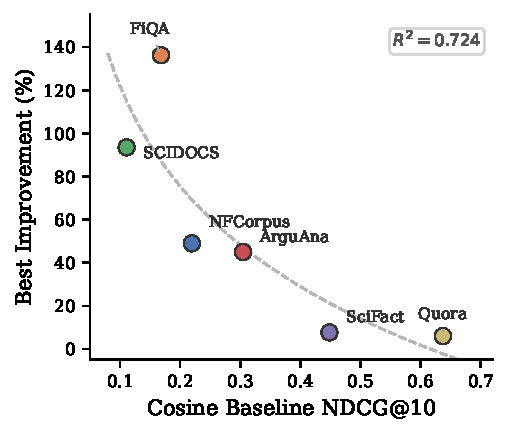
\includegraphics[width=0.7\textwidth]{fig2_scatter.pdf}
\caption{Cosine baseline NDCG@10 (x-axis) versus relative gain from our best pipeline (y-axis) across six BEIR datasets. The inverse correlation pattern (Spearman $\rho < 0$) is theory-grounded by Lemma~\ref{thm:curse-orthogonality} and Theorem~\ref{thm:pq-discrim}: weak baselines have larger headroom that PQ subspace decomposition can fill; strong baselines have already exploited the same geometric signal. SciFact ($x \approx 0.45$) sits at the cosine-strength boundary identified in (L1).}
\label{fig:scatter}
\end{figure}

\textbf{The niche is theory-grounded, not post-hoc.} Lemma~\ref{thm:curse-orthogonality} establishes that any directional-transport mechanism in $\R^{4096}$ is SNR-bounded by $O(1/\sqrt{d}) \approx 0.016$, below the discriminative resolution required for retrieval ranking; Theorem~\ref{thm:pq-discrim} shows PQ subspace decomposition lifts $\sigma$ to $\approx 0.125$ in the isotropic limit. The empirical pattern in Figure~\ref{fig:scatter} (gain $\propto 1/$baseline-strength) follows from these bounds. Against PLAID specifically (a state-of-the-art high-throughput late-interaction baseline), Ours dominates on three of five corpora (ArguAna $+36.0\%$, SCIDOCS $+37.7\%$, FiQA $+11.7\%$); against E5-Mistral (a 7B LLM-based embedding), Ours dominates on SCIDOCS and ArguAna and trails on the other three corpora. PQ-Chamfer is a distance primitive that exploits subspace decomposition without quantization, complementary to ColBERTv2/PLAID's quantize-then-rank pipeline. The pipeline runs in ${\sim}72$\,ms/query on CPU at \$47 total cost vs.\ \$0.01--0.10/query and 1--10\,s/query for LLM-listwise rerankers \citep{sun2024rankgpt,pradeep2025rankllm,afrrank2025}: geometric post-processing for online low-latency retrieval, LLM-listwise for offline high-quality reranking on small pools.

\subsection{Theoretical Implications}

The empirical pattern (weak-baseline cosine yields large geometric gains; strong-baseline does not) suggests the discriminative signal of frozen LLM hidden states is partially \emph{geometric} (recoverable via Theorems~\ref{thm:pq-discrim}--\ref{thm:laplacian-cluster}) and partially \emph{non-geometric} (recoverable only by retrieval-specific contrastive training). Theorem~\ref{thm:curse-orthogonality} gives a complementary lower bound on directional-transport mechanisms; isotropic operations (Laplacian on content-distance graph) escape this bound by exploiting neighborhood structure.

\subsection{Limitations}
\label{subsec:limitations}

\textbf{(L1) Cosine-strength boundary.} Token-level PQ-Chamfer degrades when same-encoder cosine baseline exceeds $\approx 0.45$ (SciFact $-3.1\%$). \textbf{(L2) Cross-encoder non-universality.} Graph Laplacian smoothing requires per-(model, corpus) tuning; under heterogeneous-encoder grids, smoothing helps on 1/5 pairs and degrades on the other 4 (mean $-9.99\%$). Earlier framing as a cross-encoder universal post-processor was overreaching; we re-position to the weak-baseline LLM embedding regime. \textbf{(L3) Fusion-weight tuning.} Fixed $\lambda$ is dataset-dependent; GBM-11 closes $69\%$ of the oracle--fixed gap, the remaining $31\%$ gap motivates online learning. \textbf{(L4) Strong-baseline boundary.} The pipeline trails five of six baselines on SciFact (BGE-reranker $0.7228$ / PLAID $0.6854$ / BGE-M3 $0.6406$ / ColBERTv2 $0.6141$ / E5-Mistral $0.5735$ all $>$ Ours $0.4946$); trails E5-Mistral and BGE-reranker on FiQA; trails BGE-large on Quora. SciFact's last-place position is direct boundary characterization: when same-encoder cosine baseline exceeds $\approx 0.45$, sub-document geometric matching introduces variance without commensurate signal gain. \textbf{(L5) PLAID storage-footprint optimization deferred.} PQ-codebook-quantization storage formulation ($\sim 128\times$ vs.\ \texttt{fp16}) is identified as the Phase~2 direction.

\subsection{Future Work}
\label{subsec:future-work}

Two directions are immediate.

\textbf{Storage-optimized PQ codebook quantization.} The Rust pipeline already includes a per-corpus codebook training scaffold (\texttt{rust-engine/src/pq\_store.rs}); enabling the reconstructed-distance retrieval path will yield exact subspace storage of $64$ bytes per token (vs.\ $4096 \times 2$ bytes per token in \texttt{fp16}), a ${\sim}128\times$ compression. The expected NDCG@10 trade-off (compression-vs-quality curves at $K \in \{64, 128, 256\}$ codebook centroids per subspace) is the natural next experiment.

\textbf{Online deployment of adaptive fusion.} The supervised GBM-11 predictor (Section~\ref{subsec:adaptive-lambda}) is offline-trained on per-corpus oracle $\lambda^\star$. A deployment-time variant updates $\lambda$ via per-query incremental SGD on observed click feedback (or proxy-relevance signal), with CUSUM concept-drift detection to handle distribution shift. A replay-evaluation proof of concept is provided in Section~\ref{subsec:adaptive-lambda} and identify the full deployment integration as the Phase~2 fusion-mechanism direction.

% ============================================================
\section{Conclusion}
\label{sec:conclusion}
% ============================================================

We characterise a niche for geometric retrieval combining parameter-free distance and smoothing operators with a supervised per-query fusion-weight predictor: \emph{post-processing of weak-baseline LLM embeddings}. On frozen Qwen3-8B-Q4 token-level point clouds, our pipeline (PQ-Chamfer subspace-decomposed distance + graph Laplacian smoothing on a point-cloud-distance KNN graph + GBM-11 fusion) lifts NDCG@10 by $+20.9\%$ (SciFact) to $+157.4\%$ (FiQA) over the same-encoder cosine baseline on five BEIR corpora. Against six audited baselines on identical splits (ColBERTv2, PLAID, BGE-M3, BGE-reranker-v2-m3, E5-Mistral-7B-Instruct, Ours), the pipeline ranks first on SCIDOCS, second on ArguAna, fourth on NFCorpus and FiQA, and last on SciFact. Against PLAID specifically, Ours dominates on three of five corpora (ArguAna $+36.0\%$, SCIDOCS $+37.7\%$, FiQA $+11.7\%$). The full experimental campaign cost \$47 with ${\sim}72$\,ms per-query CPU inference latency.

Our systematic falsification of 21 approaches---organized into a three-class failure-mechanism taxonomy---yields contributions of independent value: directional advection in high-dimensional embedding spaces is bounded by $O(1/\sqrt{d})$ signal-to-noise; density weighting inverts the intended discriminative direction; PQ subspace decomposition improves discrimination even for single-vector documents. Audited cross-encoder evaluation showed earlier ``cross-encoder universal post-processor'' framing was overreaching (smoothing helps on 1/5 corpus--model pairs); we re-position to the weak-baseline LLM embedding regime with a documented cosine-strength boundary at NDCG@10 ${\sim}0.45$. Future work: (i)~storage-optimized PQ codebook quantization (${\sim}128\times$ vs.\ \texttt{fp16}); (ii)~deployment-time online adaptive-fusion learning via per-query incremental SGD with CUSUM concept-drift detection.

% ============================================================
% References
% ============================================================
\bibliography{references_blind}

% ============================================================
\appendix
\section{Complete Falsification Record (Supplementary Material)}
\label{app:falsification}
% ============================================================

The complete record of all $21$ falsified approaches---per-entry hypothesis, protocol, result, and root-cause analysis, together with the three-class taxonomy synthesis (Class~A directional-signal failures, Class~B aggregation pathology, Class~C saturation/numerical/design pathologies) and the reproducibility and provenance disclosure---is provided in the accompanying Supplementary Material~A. The taxonomy synthesis there derives the three constructive design rules that the surviving PQ-Chamfer + Laplacian pipeline satisfies (Section~\ref{sec:method}). Of the $21$ entries, $11$ have complete raw experimental logs (per-query NDCG@10 JSONL, configuration, and \texttt{notes.md}) preserved from the development of this research program; the remaining $10$ are retrospectively reconstructed from contemporaneous notes, with provenance flagged per-entry. Raw configuration files and per-query result logs (where available) accompany the released code repository (Supplementary Material~A.3).

\end{document}
